\documentclass[twoside]{book}

% Packages required by doxygen
\usepackage{fixltx2e}
\usepackage{calc}
\usepackage{doxygen}
\usepackage[export]{adjustbox} % also loads graphicx
\usepackage{graphicx}
\usepackage[utf8]{inputenc}
\usepackage{makeidx}
\usepackage{multicol}
\usepackage{multirow}
\PassOptionsToPackage{warn}{textcomp}
\usepackage{textcomp}
\usepackage[nointegrals]{wasysym}
\usepackage[table]{xcolor}

% Font selection
\usepackage[T1]{fontenc}
\usepackage[scaled=.90]{helvet}
\usepackage{courier}
\usepackage{amssymb}
\usepackage{sectsty}
\renewcommand{\familydefault}{\sfdefault}
\allsectionsfont{%
  \fontseries{bc}\selectfont%
  \color{darkgray}%
}
\renewcommand{\DoxyLabelFont}{%
  \fontseries{bc}\selectfont%
  \color{darkgray}%
}
\newcommand{\+}{\discretionary{\mbox{\scriptsize$\hookleftarrow$}}{}{}}

% Page & text layout
\usepackage{geometry}
\geometry{%
  a4paper,%
  top=2.5cm,%
  bottom=2.5cm,%
  left=2.5cm,%
  right=2.5cm%
}
\tolerance=750
\hfuzz=15pt
\hbadness=750
\setlength{\emergencystretch}{15pt}
\setlength{\parindent}{0cm}
\setlength{\parskip}{3ex plus 2ex minus 2ex}
\makeatletter
\renewcommand{\paragraph}{%
  \@startsection{paragraph}{4}{0ex}{-1.0ex}{1.0ex}{%
    \normalfont\normalsize\bfseries\SS@parafont%
  }%
}
\renewcommand{\subparagraph}{%
  \@startsection{subparagraph}{5}{0ex}{-1.0ex}{1.0ex}{%
    \normalfont\normalsize\bfseries\SS@subparafont%
  }%
}
\makeatother

% Headers & footers
\usepackage{fancyhdr}
\pagestyle{fancyplain}
\fancyhead[LE]{\fancyplain{}{\bfseries\thepage}}
\fancyhead[CE]{\fancyplain{}{}}
\fancyhead[RE]{\fancyplain{}{\bfseries\leftmark}}
\fancyhead[LO]{\fancyplain{}{\bfseries\rightmark}}
\fancyhead[CO]{\fancyplain{}{}}
\fancyhead[RO]{\fancyplain{}{\bfseries\thepage}}
\fancyfoot[LE]{\fancyplain{}{}}
\fancyfoot[CE]{\fancyplain{}{}}
\fancyfoot[RE]{\fancyplain{}{\bfseries\scriptsize Generated by Doxygen }}
\fancyfoot[LO]{\fancyplain{}{\bfseries\scriptsize Generated by Doxygen }}
\fancyfoot[CO]{\fancyplain{}{}}
\fancyfoot[RO]{\fancyplain{}{}}
\renewcommand{\footrulewidth}{0.4pt}
\renewcommand{\chaptermark}[1]{%
  \markboth{#1}{}%
}
\renewcommand{\sectionmark}[1]{%
  \markright{\thesection\ #1}%
}

% Indices & bibliography
\usepackage{natbib}
\usepackage[titles]{tocloft}
\setcounter{tocdepth}{3}
\setcounter{secnumdepth}{5}
\makeindex

% Hyperlinks (required, but should be loaded last)
\usepackage{ifpdf}
\ifpdf
  \usepackage[pdftex,pagebackref=true]{hyperref}
\else
  \usepackage[ps2pdf,pagebackref=true]{hyperref}
\fi
\hypersetup{%
  colorlinks=true,%
  linkcolor=blue,%
  citecolor=blue,%
  unicode%
}

% Custom commands
\newcommand{\clearemptydoublepage}{%
  \newpage{\pagestyle{empty}\cleardoublepage}%
}

\usepackage{caption}
\captionsetup{labelsep=space,justification=centering,font={bf},singlelinecheck=off,skip=4pt,position=top}

%===== C O N T E N T S =====

\begin{document}

% Titlepage & ToC
\hypersetup{pageanchor=false,
             bookmarksnumbered=true,
             pdfencoding=unicode
            }
\pagenumbering{alph}
\begin{titlepage}
\vspace*{7cm}
\begin{center}%
{\Large Labyrinth -\/ One Player mode }\\
\vspace*{1cm}
{\large Generated by Doxygen 1.8.13}\\
\end{center}
\end{titlepage}
\clearemptydoublepage
\pagenumbering{roman}
\tableofcontents
\clearemptydoublepage
\pagenumbering{arabic}
\hypersetup{pageanchor=true}

%--- Begin generated contents ---
\chapter{Hierarchical Index}
\section{Class Hierarchy}
This inheritance list is sorted roughly, but not completely, alphabetically\+:\begin{DoxyCompactList}
\item \contentsline{section}{handle}{\pageref{classhandle}}{}
\begin{DoxyCompactList}
\item \contentsline{section}{Model\+S\+ED}{\pageref{class_model_s_e_d}}{}
\begin{DoxyCompactList}
\item \contentsline{section}{Model\+Ghost}{\pageref{class_model_ghost}}{}
\item \contentsline{section}{Model\+Laby}{\pageref{class_model_laby}}{}
\item \contentsline{section}{Model\+Pacman}{\pageref{class_model_pacman}}{}
\item \contentsline{section}{Model\+Walls}{\pageref{class_model_walls}}{}
\item \contentsline{section}{Stop\+Condition}{\pageref{class_stop_condition}}{}
\end{DoxyCompactList}
\end{DoxyCompactList}
\item \contentsline{section}{Model\+Command}{\pageref{class_model_command}}{}
\item \contentsline{section}{Wrapper}{\pageref{class_wrapper}}{}
\end{DoxyCompactList}

\chapter{Class Index}
\section{Class List}
Here are the classes, structs, unions and interfaces with brief descriptions\+:\begin{DoxyCompactList}
\item\contentsline{section}{\hyperlink{classhandle}{handle} }{\pageref{classhandle}}{}
\item\contentsline{section}{\hyperlink{class_model_command}{Model\+Command} }{\pageref{class_model_command}}{}
\item\contentsline{section}{\hyperlink{class_model_ghost}{Model\+Ghost} \\*M\+O\+D\+E\+L\+Ghost Summary of this class goes here ~\newline
 Input \+: Possible ghost\textquotesingle{}s moves \mbox{[}Up Down Left Right\mbox{]} ~\newline
 0 = move not possible ; 1 = move possible ~\newline
 ( Wout\{7\} ) ~\newline
~\newline
 Output \+: Ghost\textquotesingle{}s moves 1 \+: ghost\+Left\+But, ( Wout(3) )~\newline
 2 \+: ghost\+Up\+But, ( Wout(1) ) ~\newline
 3 \+: ghost\+Right\+But, ( Wout(4) ) ~\newline
 4 \+: ghost\+Down\+But , ( Wout(2) ) ~\newline
 ( Win( 4\+:7) of wrapper ) ~\newline
~\newline
 in\+: Walls around ghost~\newline
 1 up~\newline
 2 down~\newline
}{\pageref{class_model_ghost}}{}
\item\contentsline{section}{\hyperlink{class_model_laby}{Model\+Laby} \\*Class which contains the \char`\"{}fmg\char`\"{} structure of the labyrinth for 2 players }{\pageref{class_model_laby}}{}
\item\contentsline{section}{\hyperlink{class_model_pacman}{Model\+Pacman} \\*Input \+: Walls around Pacman ~\newline
 1 up ~\newline
 2 down~\newline
 3 left~\newline
 4 right~\newline
This command do the sequence P(\+D) $>$ P(\+B) $>$ P(\+H) $>$ P(\+G) ~\newline
}{\pageref{class_model_pacman}}{}
\item\contentsline{section}{\hyperlink{class_model_s_e_d}{Model\+S\+ED} \\*State \+: minimal information necessary who evolute }{\pageref{class_model_s_e_d}}{}
\item\contentsline{section}{\hyperlink{class_model_walls}{Model\+Walls} \\*This command do the sequence walls Right --$>$ walls down ~\newline
}{\pageref{class_model_walls}}{}
\item\contentsline{section}{\hyperlink{class_stop_condition}{Stop\+Condition} }{\pageref{class_stop_condition}}{}
\item\contentsline{section}{\hyperlink{class_wrapper}{Wrapper} }{\pageref{class_wrapper}}{}
\end{DoxyCompactList}

\chapter{File Index}
\section{File List}
Here is a list of all files with brief descriptions\+:\begin{DoxyCompactList}
\item\contentsline{section}{\hyperlink{_create_pitures_and_video_8m}{Create\+Pitures\+And\+Video.\+m} }{\pageref{_create_pitures_and_video_8m}}{}
\item\contentsline{section}{\hyperlink{_create_pitures_and_video__textured_8m}{Create\+Pitures\+And\+Video\+\_\+textured.\+m} }{\pageref{_create_pitures_and_video__textured_8m}}{}
\item\contentsline{section}{\hyperlink{figure___laby_8m}{figure\+\_\+\+Laby.\+m} }{\pageref{figure___laby_8m}}{}
\item\contentsline{section}{\hyperlink{main_8m}{main.\+m} }{\pageref{main_8m}}{}
\item\contentsline{section}{\hyperlink{_model_laby_8m}{Model\+Laby.\+m} }{\pageref{_model_laby_8m}}{}
\item\contentsline{section}{\hyperlink{_model_pacman_8m}{Model\+Pacman.\+m} \\*Contain ghost Pacman control }{\pageref{_model_pacman_8m}}{}
\item\contentsline{section}{\hyperlink{_model_s_e_d_8m}{Model\+S\+E\+D.\+m} \\*Abstract Class who contain the structure of a \char`\"{}fmg\char`\"{} implementation }{\pageref{_model_s_e_d_8m}}{}
\item\contentsline{section}{\hyperlink{_model_walls_8m}{Model\+Walls.\+m} \\*Contain wall movement command }{\pageref{_model_walls_8m}}{}
\item\contentsline{section}{\hyperlink{set_color_8m}{set\+Color.\+m} }{\pageref{set_color_8m}}{}
\item\contentsline{section}{\hyperlink{_simulation_8m}{Simulation.\+m} }{\pageref{_simulation_8m}}{}
\item\contentsline{section}{\hyperlink{_stop_condition_8m}{Stop\+Condition.\+m} }{\pageref{_stop_condition_8m}}{}
\item\contentsline{section}{\hyperlink{visupacman_8m}{visupacman.\+m} }{\pageref{visupacman_8m}}{}
\item\contentsline{section}{\hyperlink{visupacman2_8m}{visupacman2.\+m} }{\pageref{visupacman2_8m}}{}
\item\contentsline{section}{\hyperlink{walls_border_8m}{walls\+Border.\+m} }{\pageref{walls_border_8m}}{}
\item\contentsline{section}{\hyperlink{_wrapper_8m}{Wrapper.\+m} }{\pageref{_wrapper_8m}}{}
\item\contentsline{section}{automaton/\hyperlink{_automate_graph_8m}{Automate\+Graph.\+m} }{\pageref{_automate_graph_8m}}{}
\item\contentsline{section}{automaton/\hyperlink{main_laby_8m}{main\+Laby.\+m} }{\pageref{main_laby_8m}}{}
\item\contentsline{section}{automaton/\hyperlink{_parrallel_composition_8m}{Parrallel\+Composition.\+m} }{\pageref{_parrallel_composition_8m}}{}
\item\contentsline{section}{automaton/model\+Generator/\hyperlink{_automaton_scheduling_creation_8m}{Automaton\+Scheduling\+Creation.\+m} }{\pageref{_automaton_scheduling_creation_8m}}{}
\item\contentsline{section}{automaton/model\+Generator/\hyperlink{_automaton_struture_laby_creation_8m}{Automaton\+Struture\+Laby\+Creation.\+m} }{\pageref{_automaton_struture_laby_creation_8m}}{}
\item\contentsline{section}{automaton/model\+Generator/\hyperlink{_automaton_walls_contraints_creation_8m}{Automaton\+Walls\+Contraints\+Creation.\+m} }{\pageref{_automaton_walls_contraints_creation_8m}}{}
\item\contentsline{section}{automaton/model\+Generator/\hyperlink{generer__lab_8m}{generer\+\_\+lab.\+m} }{\pageref{generer__lab_8m}}{}
\item\contentsline{section}{automaton/model\+Generator/\hyperlink{model_generator_8m}{model\+Generator.\+m} }{\pageref{model_generator_8m}}{}
\item\contentsline{section}{automaton/model\+Generator/\hyperlink{_plan__desuma_functions_8m}{Plan\+\_\+desuma\+Functions.\+m} }{\pageref{_plan__desuma_functions_8m}}{}
\item\contentsline{section}{automaton/model\+Generator/\hyperlink{_save_d_e_s_u_m_a_file_8m}{Save\+D\+E\+S\+U\+M\+A\+File.\+m} }{\pageref{_save_d_e_s_u_m_a_file_8m}}{}
\item\contentsline{section}{automaton/model\+Generator/\hyperlink{write_states_8m}{write\+States.\+m} }{\pageref{write_states_8m}}{}
\item\contentsline{section}{automaton/model\+Generator/\hyperlink{write_transitions_8m}{write\+Transitions.\+m} }{\pageref{write_transitions_8m}}{}
\item\contentsline{section}{automaton/optimal\+Command/\hyperlink{creation_matricetransition_8m}{creation\+Matricetransition.\+m} }{\pageref{creation_matricetransition_8m}}{}
\item\contentsline{section}{automaton/optimal\+Command/\hyperlink{get_state_transition_f_s_m_8m}{get\+State\+Transition\+F\+S\+M.\+m} }{\pageref{get_state_transition_f_s_m_8m}}{}
\item\contentsline{section}{automaton/optimal\+Command/\hyperlink{get_state_transition_t_x_t_8m}{get\+State\+Transition\+T\+X\+T.\+m} }{\pageref{get_state_transition_t_x_t_8m}}{}
\item\contentsline{section}{automaton/optimal\+Command/\hyperlink{automaton_2optimal_command_2main_8m}{main.\+m} }{\pageref{automaton_2optimal_command_2main_8m}}{}
\item\contentsline{section}{automaton/optimal\+Command/\hyperlink{optimal_command_8m}{optimal\+Command.\+m} }{\pageref{optimal_command_8m}}{}
\item\contentsline{section}{automaton/optimal\+Command/\hyperlink{_parcourir_matrices_transitions_8m}{Parcourir\+Matrices\+Transitions.\+m} }{\pageref{_parcourir_matrices_transitions_8m}}{}
\item\contentsline{section}{automaton/optimal\+Command/\hyperlink{rafine_automaton_8m}{rafine\+Automaton.\+m} }{\pageref{rafine_automaton_8m}}{}
\item\contentsline{section}{automaton/optimal\+Command/\hyperlink{rafine_automaton_class_8m}{rafine\+Automaton\+Class.\+m} }{\pageref{rafine_automaton_class_8m}}{}
\item\contentsline{section}{automaton\+\_\+nd/\hyperlink{_automaton_8m}{Automaton.\+m} }{\pageref{_automaton_8m}}{}
\item\contentsline{section}{automaton\+\_\+nd/\hyperlink{_labyrinthe_8m}{Labyrinthe.\+m} }{\pageref{_labyrinthe_8m}}{}
\item\contentsline{section}{automaton\+\_\+nd/\hyperlink{modi__main_8m}{modi\+\_\+main.\+m} }{\pageref{modi__main_8m}}{}
\end{DoxyCompactList}

\chapter{Class Documentation}
\hypertarget{classhandle}{}\section{handle Class Reference}
\label{classhandle}\index{handle@{handle}}


Inheritance diagram for handle\+:
\nopagebreak
\begin{figure}[H]
\begin{center}
\leavevmode
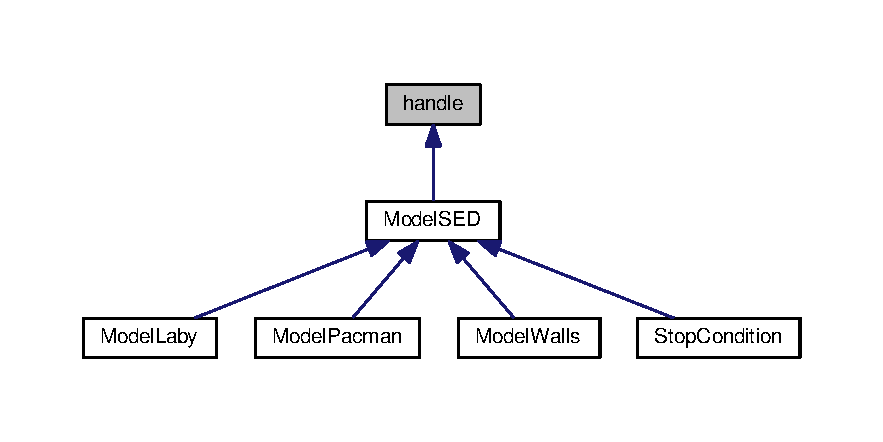
\includegraphics[width=350pt]{classhandle__inherit__graph}
\end{center}
\end{figure}


The documentation for this class was generated from the following file\+:\begin{DoxyCompactItemize}
\item 
\hyperlink{_model_s_e_d_8m}{Model\+S\+E\+D.\+m}\end{DoxyCompactItemize}

\hypertarget{class_model_laby}{}\section{Model\+Laby Class Reference}
\label{class_model_laby}\index{Model\+Laby@{Model\+Laby}}


Class which contains the \char`\"{}fmg\char`\"{} structure of the labyrinth for 2 players.  




Inheritance diagram for Model\+Laby\+:
\nopagebreak
\begin{figure}[H]
\begin{center}
\leavevmode
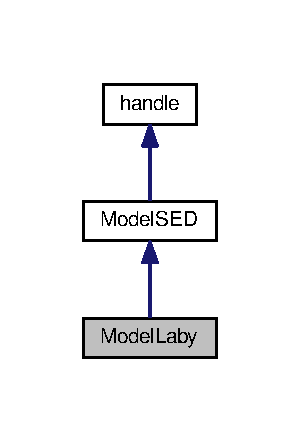
\includegraphics[width=144pt]{class_model_laby__inherit__graph}
\end{center}
\end{figure}


Collaboration diagram for Model\+Laby\+:
\nopagebreak
\begin{figure}[H]
\begin{center}
\leavevmode
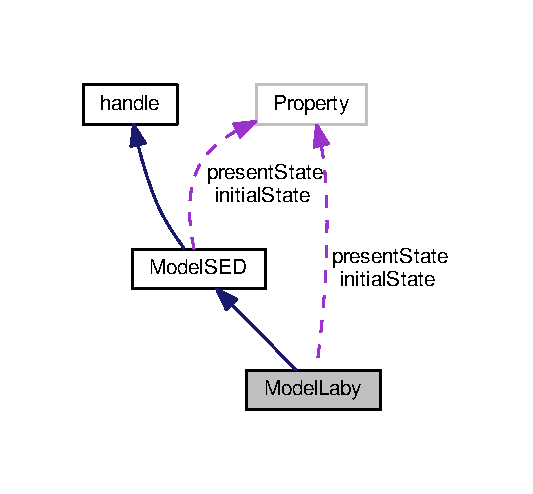
\includegraphics[width=256pt]{class_model_laby__coll__graph}
\end{center}
\end{figure}
\subsection*{Public Member Functions}
\begin{DoxyCompactItemize}
\item 
\hyperlink{_plan__desuma_functions__2_players_8m_ac2ffb26d6f42d3bbcd7847b0873403f4}{function} \hyperlink{class_model_laby_a014d91cfa3ecf1a6fc3ca75ea4f433d4}{Model\+Laby} (in walls\+V\+\_\+init, in walls\+H\+\_\+init, in pacman\+\_\+init, in ghost\+\_\+init, in escape\+\_\+init, in caught\+\_\+init)
\begin{DoxyCompactList}\small\item\em Class constructor of. \end{DoxyCompactList}\item 
\hyperlink{_plan__desuma_functions__2_players_8m_ac2ffb26d6f42d3bbcd7847b0873403f4}{function} \hyperlink{class_model_laby_a6f3b146c92a207e95690d08975e1e072}{f} (in obj, in in)
\begin{DoxyCompactList}\small\item\em Compute the evolution of the model. \end{DoxyCompactList}\item 
\hyperlink{_plan__desuma_functions__2_players_8m_ac2ffb26d6f42d3bbcd7847b0873403f4}{function} \hyperlink{class_model_laby_a3140f24c6c4b80037b7d4f521c6ae2d3}{m} (in obj, in next\+State, in init)
\begin{DoxyCompactList}\small\item\em Memory method update the state of the command. \end{DoxyCompactList}\item 
\hyperlink{_plan__desuma_functions__2_players_8m_ac2ffb26d6f42d3bbcd7847b0873403f4}{function} \hyperlink{class_model_laby_a07dadfabe92bf9a144b8a862720e7746}{g} (in obj)
\begin{DoxyCompactList}\small\item\em Create the outputs in a 1x9 cell-\/array. \end{DoxyCompactList}\item 
\hyperlink{_plan__desuma_functions__2_players_8m_ac2ffb26d6f42d3bbcd7847b0873403f4}{function} \hyperlink{class_model_laby_ac2632946f3f89dcc57c9f1fd31bbfb53}{same\+X\+\_\+position} (in obj)
\begin{DoxyCompactList}\small\item\em Method to analyze Ghost and Pacman Position. \end{DoxyCompactList}\item 
\hyperlink{_plan__desuma_functions__2_players_8m_ac2ffb26d6f42d3bbcd7847b0873403f4}{function} \hyperlink{class_model_laby_a104c64766fa031eb4a29214f07da63d2}{same\+Y\+\_\+position} (in obj)
\begin{DoxyCompactList}\small\item\em Method to analyze Ghost and Pacman Position. \end{DoxyCompactList}\item 
\hyperlink{_plan__desuma_functions__2_players_8m_ac2ffb26d6f42d3bbcd7847b0873403f4}{function} \hyperlink{class_model_laby_adf2ec45a05676923165cb7f273900569}{walls\+V\+Between} (in obj, in obj1, in obj2)
\begin{DoxyCompactList}\small\item\em Method to analyze if a Vertical wall is between 2 objects. \end{DoxyCompactList}\item 
\hyperlink{_plan__desuma_functions__2_players_8m_ac2ffb26d6f42d3bbcd7847b0873403f4}{function} \hyperlink{class_model_laby_a488955f2ead0854b15302161753a0a66}{walls\+H\+Between} (in obj, in obj1, in obj2)
\begin{DoxyCompactList}\small\item\em Method to analyze if a Horizontal wall is between 2 objects. \end{DoxyCompactList}\item 
\hyperlink{_plan__desuma_functions__2_players_8m_ac2ffb26d6f42d3bbcd7847b0873403f4}{function} \hyperlink{class_model_laby_ab8486279acbf0a66424a84fa210d1b71}{walls\+V\+Between\+One} (in obj, in obj1, in obj2)
\begin{DoxyCompactList}\small\item\em Method to analyze if a Horizontal wall is between 2 objects side by side. \end{DoxyCompactList}\item 
\hyperlink{_plan__desuma_functions__2_players_8m_ac2ffb26d6f42d3bbcd7847b0873403f4}{function} \hyperlink{class_model_laby_a450d4d89542d177b6676375984146f4c}{walls\+H\+Between\+One} (in obj, in obj1, in obj2)
\begin{DoxyCompactList}\small\item\em Method to analyze if a Horizontal wall is between 2 objects side by side. \end{DoxyCompactList}\end{DoxyCompactItemize}
\subsection*{Public Attributes}
\begin{DoxyCompactItemize}
\item 
Property \hyperlink{class_model_laby_a9624cc7c421a50fa5086b0ebd0cd5fe3}{present\+State}
\begin{DoxyCompactList}\small\item\em Data Structure of the current state of Labyrinth. ~\newline
 It contains \char`\"{}walls\+V\char`\"{}, \char`\"{}walls\+H\char`\"{} (2 matrix for the walls), \char`\"{}ghost\char`\"{}, \char`\"{}pacman\char`\"{} and \char`\"{}escape\char`\"{} , a Cartesian position of current position of ghost, pacman and escape. ~\newline
 There is also 3 vectors \+: \textquotesingle{}walls\+Around\+Pacman\textquotesingle{}, \textquotesingle{}walls\+Around\+Ghost\textquotesingle{} and \textquotesingle{}ghost\+Sees\+Pacman\textquotesingle{} A vector indicating the presence of a wall around the Pacman and ghost for the 4 directions Up Down Left Right. \end{DoxyCompactList}\item 
Property \hyperlink{class_model_laby_acd9263acfa96c9138afdf497e55acc24}{initial\+State}
\begin{DoxyCompactList}\small\item\em Data Structure of the initial state of Labyrinth. It contains \char`\"{}walls\+V\char`\"{}, \char`\"{}walls\+H\char`\"{} (2 matrix for the walls), \char`\"{}escape\char`\"{} and \char`\"{}pacman\char`\"{}, a Cartesian position of current position of escape and pacman and \textquotesingle{}walls\+Around\+Pacman\textquotesingle{} A vector indicating the presence of a wall around the Pacman for the 4 directions Up Down Left Right. \end{DoxyCompactList}\end{DoxyCompactItemize}


\subsection{Detailed Description}
Class which contains the \char`\"{}fmg\char`\"{} structure of the labyrinth for 2 players. 

You can change here labyrinth\textquotesingle{}s dynamic \+: how objects and walls are evolving in the labyrinth, not the command of then.~\newline
 Input \+: necessary information for compute the next state of the model~\newline
~\newline
 Output \+: output\textquotesingle{}s action of the model~\newline
 ~\newline
 State \+: minimal information necessary who evolute 

\subsection{Constructor \& Destructor Documentation}
\mbox{\Hypertarget{class_model_laby_a014d91cfa3ecf1a6fc3ca75ea4f433d4}\label{class_model_laby_a014d91cfa3ecf1a6fc3ca75ea4f433d4}} 
\index{Model\+Laby@{Model\+Laby}!Model\+Laby@{Model\+Laby}}
\index{Model\+Laby@{Model\+Laby}!Model\+Laby@{Model\+Laby}}
\subsubsection{\texorpdfstring{Model\+Laby()}{ModelLaby()}}
{\footnotesize\ttfamily \hyperlink{_plan__desuma_functions__2_players_8m_ac2ffb26d6f42d3bbcd7847b0873403f4}{function} \hyperlink{class_model_laby}{Model\+Laby} (\begin{DoxyParamCaption}\item[{in}]{walls\+V\+\_\+init,  }\item[{in}]{walls\+H\+\_\+init,  }\item[{in}]{pacman\+\_\+init,  }\item[{in}]{ghost\+\_\+init,  }\item[{in}]{escape\+\_\+init,  }\item[{in}]{caught\+\_\+init }\end{DoxyParamCaption})}



Class constructor of. 


\begin{DoxyParams}{Parameters}
{\em walls\+V\+\_\+init} & Contain a matrix (N, N-\/1) of Initial Vertical Walls. \\
\hline
{\em walls\+H\+\_\+init} & Contain a matrix (N-\/1, N) of Initial Horizontal Walls. \\
\hline
{\em pacman\+\_\+init} & Contain a vector (x, y) of Initial Position of Pacman. \\
\hline
{\em pacman\+\_\+init} & Contain a vector (x, y) of Initial Position of Ghost. \\
\hline
{\em escape\+\_\+init} & Contain a vector (x, y) of Escape \textquotesingle{}s Position. \\
\hline
{\em caught\+\_\+init} & Contain a integer of the number of times the Pacman was caught by the ghost. \\
\hline
\end{DoxyParams}
\begin{DoxyReturn}{Returns}
instance of the \hyperlink{class_model_laby}{Model\+Laby} class. 
\end{DoxyReturn}


\subsection{Member Function Documentation}
\mbox{\Hypertarget{class_model_laby_a6f3b146c92a207e95690d08975e1e072}\label{class_model_laby_a6f3b146c92a207e95690d08975e1e072}} 
\index{Model\+Laby@{Model\+Laby}!f@{f}}
\index{f@{f}!Model\+Laby@{Model\+Laby}}
\subsubsection{\texorpdfstring{f()}{f()}}
{\footnotesize\ttfamily \hyperlink{_plan__desuma_functions__2_players_8m_ac2ffb26d6f42d3bbcd7847b0873403f4}{function} f (\begin{DoxyParamCaption}\item[{in}]{obj,  }\item[{in}]{in }\end{DoxyParamCaption})\hspace{0.3cm}{\ttfamily [virtual]}}



Compute the evolution of the model. 


\begin{DoxyParams}{Parameters}
{\em obj} & The instance which will evolve. \\
\hline
{\em in} & Input needed for the computing. \\
\hline
\end{DoxyParams}

\begin{DoxyRetVals}{Return values}
{\em next\+State} & Next instance of the \hyperlink{class_model_laby}{Model\+Laby} class. \\
\hline
\end{DoxyRetVals}


Reimplemented from \hyperlink{class_model_s_e_d_ac36f9451c43b120828af4380858f2024}{Model\+S\+ED}.

\mbox{\Hypertarget{class_model_laby_a07dadfabe92bf9a144b8a862720e7746}\label{class_model_laby_a07dadfabe92bf9a144b8a862720e7746}} 
\index{Model\+Laby@{Model\+Laby}!g@{g}}
\index{g@{g}!Model\+Laby@{Model\+Laby}}
\subsubsection{\texorpdfstring{g()}{g()}}
{\footnotesize\ttfamily \hyperlink{_plan__desuma_functions__2_players_8m_ac2ffb26d6f42d3bbcd7847b0873403f4}{function} g (\begin{DoxyParamCaption}\item[{in}]{obj }\end{DoxyParamCaption})\hspace{0.3cm}{\ttfamily [virtual]}}



Create the outputs in a 1x9 cell-\/array. 


\begin{DoxyParams}{Parameters}
{\em obj} & the concerned instance of the class \\
\hline
\end{DoxyParams}

\begin{DoxyRetVals}{Return values}
{\em out} & Constructed output 1x9 cell-\/array of the model \\
\hline
\end{DoxyRetVals}


Reimplemented from \hyperlink{class_model_s_e_d_ac6bf71081e35755d5ed9992d165afcb8}{Model\+S\+ED}.

\mbox{\Hypertarget{class_model_laby_a3140f24c6c4b80037b7d4f521c6ae2d3}\label{class_model_laby_a3140f24c6c4b80037b7d4f521c6ae2d3}} 
\index{Model\+Laby@{Model\+Laby}!m@{m}}
\index{m@{m}!Model\+Laby@{Model\+Laby}}
\subsubsection{\texorpdfstring{m()}{m()}}
{\footnotesize\ttfamily \hyperlink{_plan__desuma_functions__2_players_8m_ac2ffb26d6f42d3bbcd7847b0873403f4}{function} m (\begin{DoxyParamCaption}\item[{in}]{obj,  }\item[{in}]{next\+State,  }\item[{in}]{init }\end{DoxyParamCaption})\hspace{0.3cm}{\ttfamily [virtual]}}



Memory method update the state of the command. 


\begin{DoxyParams}{Parameters}
{\em obj} & The selected instance of the class \\
\hline
{\em next\+State} & The value of the state need to update \\
\hline
{\em init} & Boolean condition for initialize or reset the command \\
\hline
\end{DoxyParams}
\begin{DoxyReturn}{Returns}
instance of the class updated 
\end{DoxyReturn}


Reimplemented from \hyperlink{class_model_s_e_d_adb8aaccb857cf5bbec640cd00915459d}{Model\+S\+ED}.

\mbox{\Hypertarget{class_model_laby_ac2632946f3f89dcc57c9f1fd31bbfb53}\label{class_model_laby_ac2632946f3f89dcc57c9f1fd31bbfb53}} 
\index{Model\+Laby@{Model\+Laby}!same\+X\+\_\+position@{same\+X\+\_\+position}}
\index{same\+X\+\_\+position@{same\+X\+\_\+position}!Model\+Laby@{Model\+Laby}}
\subsubsection{\texorpdfstring{same\+X\+\_\+position()}{sameX\_position()}}
{\footnotesize\ttfamily \hyperlink{_plan__desuma_functions__2_players_8m_ac2ffb26d6f42d3bbcd7847b0873403f4}{function} same\+X\+\_\+position (\begin{DoxyParamCaption}\item[{in}]{obj }\end{DoxyParamCaption})}



Method to analyze Ghost and Pacman Position. 


\begin{DoxyParams}{Parameters}
{\em obj} & Current Instance of the Labyrinth  1 if ghost and Pacman are on the same X colon \\
\hline
\end{DoxyParams}
\mbox{\Hypertarget{class_model_laby_a104c64766fa031eb4a29214f07da63d2}\label{class_model_laby_a104c64766fa031eb4a29214f07da63d2}} 
\index{Model\+Laby@{Model\+Laby}!same\+Y\+\_\+position@{same\+Y\+\_\+position}}
\index{same\+Y\+\_\+position@{same\+Y\+\_\+position}!Model\+Laby@{Model\+Laby}}
\subsubsection{\texorpdfstring{same\+Y\+\_\+position()}{sameY\_position()}}
{\footnotesize\ttfamily \hyperlink{_plan__desuma_functions__2_players_8m_ac2ffb26d6f42d3bbcd7847b0873403f4}{function} same\+Y\+\_\+position (\begin{DoxyParamCaption}\item[{in}]{obj }\end{DoxyParamCaption})}



Method to analyze Ghost and Pacman Position. 


\begin{DoxyParams}{Parameters}
{\em obj} & Current Instance of the Labyrinth  1 if ghost and Pacman are on the same Y line \\
\hline
\end{DoxyParams}
\mbox{\Hypertarget{class_model_laby_a488955f2ead0854b15302161753a0a66}\label{class_model_laby_a488955f2ead0854b15302161753a0a66}} 
\index{Model\+Laby@{Model\+Laby}!walls\+H\+Between@{walls\+H\+Between}}
\index{walls\+H\+Between@{walls\+H\+Between}!Model\+Laby@{Model\+Laby}}
\subsubsection{\texorpdfstring{walls\+H\+Between()}{wallsHBetween()}}
{\footnotesize\ttfamily \hyperlink{_plan__desuma_functions__2_players_8m_ac2ffb26d6f42d3bbcd7847b0873403f4}{function} walls\+H\+Between (\begin{DoxyParamCaption}\item[{in}]{obj,  }\item[{in}]{obj1,  }\item[{in}]{obj2 }\end{DoxyParamCaption})}



Method to analyze if a Horizontal wall is between 2 objects. 


\begin{DoxyParams}{Parameters}
{\em obj} & Current Instance of the Labyrinth \\
\hline
{\em obj1} & Cartesian position of object 1 \\
\hline
{\em obj2} & Cartesian position of object 2  1 if there No Horizontal wall Between Object 1 and Object 2 \\
\hline
\end{DoxyParams}
\mbox{\Hypertarget{class_model_laby_a450d4d89542d177b6676375984146f4c}\label{class_model_laby_a450d4d89542d177b6676375984146f4c}} 
\index{Model\+Laby@{Model\+Laby}!walls\+H\+Between\+One@{walls\+H\+Between\+One}}
\index{walls\+H\+Between\+One@{walls\+H\+Between\+One}!Model\+Laby@{Model\+Laby}}
\subsubsection{\texorpdfstring{walls\+H\+Between\+One()}{wallsHBetweenOne()}}
{\footnotesize\ttfamily \hyperlink{_plan__desuma_functions__2_players_8m_ac2ffb26d6f42d3bbcd7847b0873403f4}{function} walls\+H\+Between\+One (\begin{DoxyParamCaption}\item[{in}]{obj,  }\item[{in}]{obj1,  }\item[{in}]{obj2 }\end{DoxyParamCaption})}



Method to analyze if a Horizontal wall is between 2 objects side by side. 


\begin{DoxyParams}{Parameters}
{\em obj} & Current Instance of the Labyrinth \\
\hline
{\em obj1} & Cartesian position of object 1 \\
\hline
{\em obj2} & Cartesian position of object 2  1 if there No Horizontal wall Between Object 1 and Object 2 \\
\hline
\end{DoxyParams}
\mbox{\Hypertarget{class_model_laby_adf2ec45a05676923165cb7f273900569}\label{class_model_laby_adf2ec45a05676923165cb7f273900569}} 
\index{Model\+Laby@{Model\+Laby}!walls\+V\+Between@{walls\+V\+Between}}
\index{walls\+V\+Between@{walls\+V\+Between}!Model\+Laby@{Model\+Laby}}
\subsubsection{\texorpdfstring{walls\+V\+Between()}{wallsVBetween()}}
{\footnotesize\ttfamily \hyperlink{_plan__desuma_functions__2_players_8m_ac2ffb26d6f42d3bbcd7847b0873403f4}{function} walls\+V\+Between (\begin{DoxyParamCaption}\item[{in}]{obj,  }\item[{in}]{obj1,  }\item[{in}]{obj2 }\end{DoxyParamCaption})}



Method to analyze if a Vertical wall is between 2 objects. 


\begin{DoxyParams}{Parameters}
{\em obj} & Current Instance of the Labyrinth \\
\hline
{\em obj1} & Cartesian position of object 1 \\
\hline
{\em obj2} & Cartesian position of object 2  1 if there No Vertical wall Between Object 1 and Object 2 \\
\hline
\end{DoxyParams}
\mbox{\Hypertarget{class_model_laby_ab8486279acbf0a66424a84fa210d1b71}\label{class_model_laby_ab8486279acbf0a66424a84fa210d1b71}} 
\index{Model\+Laby@{Model\+Laby}!walls\+V\+Between\+One@{walls\+V\+Between\+One}}
\index{walls\+V\+Between\+One@{walls\+V\+Between\+One}!Model\+Laby@{Model\+Laby}}
\subsubsection{\texorpdfstring{walls\+V\+Between\+One()}{wallsVBetweenOne()}}
{\footnotesize\ttfamily \hyperlink{_plan__desuma_functions__2_players_8m_ac2ffb26d6f42d3bbcd7847b0873403f4}{function} walls\+V\+Between\+One (\begin{DoxyParamCaption}\item[{in}]{obj,  }\item[{in}]{obj1,  }\item[{in}]{obj2 }\end{DoxyParamCaption})}



Method to analyze if a Horizontal wall is between 2 objects side by side. 


\begin{DoxyParams}{Parameters}
{\em obj} & Current Instance of the Labyrinth \\
\hline
{\em obj1} & Cartesian position of object 1 \\
\hline
{\em obj2} & Cartesian position of object 2  1 if there No Horizontal wall Between Object 1 and Object 2 \\
\hline
\end{DoxyParams}


\subsection{Member Data Documentation}
\mbox{\Hypertarget{class_model_laby_acd9263acfa96c9138afdf497e55acc24}\label{class_model_laby_acd9263acfa96c9138afdf497e55acc24}} 
\index{Model\+Laby@{Model\+Laby}!initial\+State@{initial\+State}}
\index{initial\+State@{initial\+State}!Model\+Laby@{Model\+Laby}}
\subsubsection{\texorpdfstring{initial\+State}{initialState}}
{\footnotesize\ttfamily Property initial\+State}



Data Structure of the initial state of Labyrinth. It contains \char`\"{}walls\+V\char`\"{}, \char`\"{}walls\+H\char`\"{} (2 matrix for the walls), \char`\"{}escape\char`\"{} and \char`\"{}pacman\char`\"{}, a Cartesian position of current position of escape and pacman and \textquotesingle{}walls\+Around\+Pacman\textquotesingle{} A vector indicating the presence of a wall around the Pacman for the 4 directions Up Down Left Right. 

\mbox{\Hypertarget{class_model_laby_a9624cc7c421a50fa5086b0ebd0cd5fe3}\label{class_model_laby_a9624cc7c421a50fa5086b0ebd0cd5fe3}} 
\index{Model\+Laby@{Model\+Laby}!present\+State@{present\+State}}
\index{present\+State@{present\+State}!Model\+Laby@{Model\+Laby}}
\subsubsection{\texorpdfstring{present\+State}{presentState}}
{\footnotesize\ttfamily Property present\+State}



Data Structure of the current state of Labyrinth. ~\newline
 It contains \char`\"{}walls\+V\char`\"{}, \char`\"{}walls\+H\char`\"{} (2 matrix for the walls), \char`\"{}ghost\char`\"{}, \char`\"{}pacman\char`\"{} and \char`\"{}escape\char`\"{} , a Cartesian position of current position of ghost, pacman and escape. ~\newline
 There is also 3 vectors \+: \textquotesingle{}walls\+Around\+Pacman\textquotesingle{}, \textquotesingle{}walls\+Around\+Ghost\textquotesingle{} and \textquotesingle{}ghost\+Sees\+Pacman\textquotesingle{} A vector indicating the presence of a wall around the Pacman and ghost for the 4 directions Up Down Left Right. 



The documentation for this class was generated from the following file\+:\begin{DoxyCompactItemize}
\item 
\hyperlink{_model_laby_8m}{Model\+Laby.\+m}\end{DoxyCompactItemize}

\hypertarget{class_model_pacman}{}\section{Model\+Pacman Class Reference}
\label{class_model_pacman}\index{Model\+Pacman@{Model\+Pacman}}


Input \+: Possible Pacman\textquotesingle{}s moves \mbox{[}Up Down Left Right\mbox{]} ~\newline
 0 = move not possible ; 1 = move possible ~\newline
 ( Wout\{7\} )~\newline
~\newline
 Output \+: Pacman\textquotesingle{}s moves 1 \+: pacman\+Left\+But, ( Wout(3) )~\newline
 2 \+: pacman\+Up\+But, ( Wout(1) )~\newline
 3 \+: pacman\+Right\+But, ( Wout(4) )~\newline
 4 \+: pacman\+Down\+But , ( Wout(2) )~\newline
 ( Win( 4\+:7) of wrapper ) ~\newline
.  




Inheritance diagram for Model\+Pacman\+:\nopagebreak
\begin{figure}[H]
\begin{center}
\leavevmode
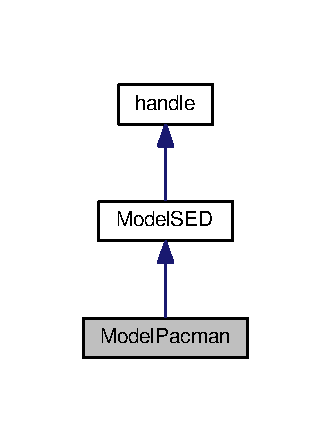
\includegraphics[width=159pt]{class_model_pacman__inherit__graph}
\end{center}
\end{figure}


Collaboration diagram for Model\+Pacman\+:\nopagebreak
\begin{figure}[H]
\begin{center}
\leavevmode
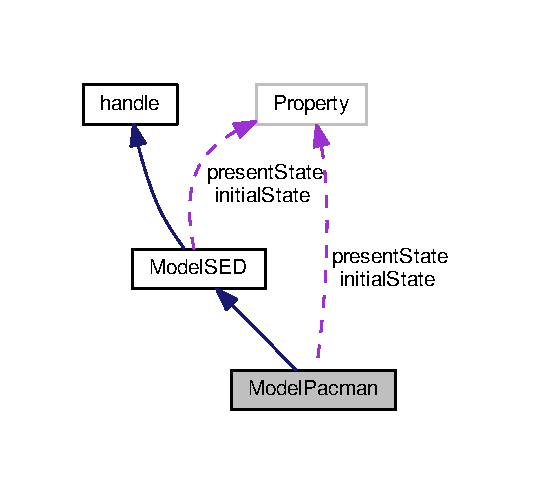
\includegraphics[width=253pt]{class_model_pacman__coll__graph}
\end{center}
\end{figure}
\subsection*{Public Member Functions}
\begin{DoxyCompactItemize}
\item 
\hyperlink{_plan__desuma_functions__2_players_8m_ac2ffb26d6f42d3bbcd7847b0873403f4}{function} \hyperlink{class_model_pacman_aeece945de8fe29ca408290f87392ac3d}{Model\+Pacman} (in initial\+Value)
\begin{DoxyCompactList}\small\item\em Class constructor. \end{DoxyCompactList}\item 
\hyperlink{_plan__desuma_functions__2_players_8m_ac2ffb26d6f42d3bbcd7847b0873403f4}{function} \hyperlink{class_model_pacman_a6f3b146c92a207e95690d08975e1e072}{f} (in obj, in in)
\begin{DoxyCompactList}\small\item\em Compute the evolution of the command. \end{DoxyCompactList}\item 
\hyperlink{_plan__desuma_functions__2_players_8m_ac2ffb26d6f42d3bbcd7847b0873403f4}{function} \hyperlink{class_model_pacman_a3140f24c6c4b80037b7d4f521c6ae2d3}{m} (in obj, in next\+State, in init)
\begin{DoxyCompactList}\small\item\em Memory method update the state of the command. \end{DoxyCompactList}\item 
\hyperlink{_plan__desuma_functions__2_players_8m_ac2ffb26d6f42d3bbcd7847b0873403f4}{function} \hyperlink{class_model_pacman_a07dadfabe92bf9a144b8a862720e7746}{g} (in obj)
\begin{DoxyCompactList}\small\item\em Create the outputs. \end{DoxyCompactList}\end{DoxyCompactItemize}
\subsection*{Public Attributes}
\begin{DoxyCompactItemize}
\item 
Property \hyperlink{class_model_pacman_a9624cc7c421a50fa5086b0ebd0cd5fe3}{present\+State}
\begin{DoxyCompactList}\small\item\em This is the state of the command in the present moment. \end{DoxyCompactList}\item 
Property \hyperlink{class_model_pacman_acd9263acfa96c9138afdf497e55acc24}{initial\+State}
\begin{DoxyCompactList}\small\item\em This is the state of the command in the initialization and when it\textquotesingle{}s reseted. \end{DoxyCompactList}\item 
Property \hyperlink{class_model_pacman_a9a61c54203464d470acd8580a6464f8e}{memory}
\begin{DoxyCompactList}\small\item\em This is another state who deed to be include. \end{DoxyCompactList}\item 
Property \hyperlink{class_model_pacman_a103c618d75e54c3a72fac6bcaa59f61f}{i}
\end{DoxyCompactItemize}


\subsection{Detailed Description}
Input \+: Possible Pacman\textquotesingle{}s moves \mbox{[}Up Down Left Right\mbox{]} ~\newline
 0 = move not possible ; 1 = move possible ~\newline
 ( Wout\{7\} )~\newline
~\newline
 Output \+: Pacman\textquotesingle{}s moves 1 \+: pacman\+Left\+But, ( Wout(3) )~\newline
 2 \+: pacman\+Up\+But, ( Wout(1) )~\newline
 3 \+: pacman\+Right\+But, ( Wout(4) )~\newline
 4 \+: pacman\+Down\+But , ( Wout(2) )~\newline
 ( Win( 4\+:7) of wrapper ) ~\newline
. 

Input \+: Walls around Pacman ~\newline
 1 up ~\newline
 2 down~\newline
 3 left~\newline
 4 right~\newline
This command do the sequence P(\+D) $>$ P(\+B) $>$ P(\+H) $>$ P(\+G) ~\newline
 

\subsection{Constructor \& Destructor Documentation}
\mbox{\Hypertarget{class_model_pacman_aeece945de8fe29ca408290f87392ac3d}\label{class_model_pacman_aeece945de8fe29ca408290f87392ac3d}} 
\index{Model\+Pacman@{Model\+Pacman}!Model\+Pacman@{Model\+Pacman}}
\index{Model\+Pacman@{Model\+Pacman}!Model\+Pacman@{Model\+Pacman}}
\subsubsection{\texorpdfstring{Model\+Pacman()}{ModelPacman()}}
{\footnotesize\ttfamily \hyperlink{_plan__desuma_functions__2_players_8m_ac2ffb26d6f42d3bbcd7847b0873403f4}{function} \hyperlink{class_model_pacman}{Model\+Pacman} (\begin{DoxyParamCaption}\item[{in}]{initial\+Value }\end{DoxyParamCaption})}



Class constructor. 


\begin{DoxyParams}{Parameters}
{\em initial\+Value} & Contain the initial state \\
\hline
\end{DoxyParams}
\begin{DoxyReturn}{Returns}
instance of the \hyperlink{class_model_pacman}{Model\+Pacman} class. 
\end{DoxyReturn}


\subsection{Member Function Documentation}
\mbox{\Hypertarget{class_model_pacman_a6f3b146c92a207e95690d08975e1e072}\label{class_model_pacman_a6f3b146c92a207e95690d08975e1e072}} 
\index{Model\+Pacman@{Model\+Pacman}!f@{f}}
\index{f@{f}!Model\+Pacman@{Model\+Pacman}}
\subsubsection{\texorpdfstring{f()}{f()}}
{\footnotesize\ttfamily \hyperlink{_plan__desuma_functions__2_players_8m_ac2ffb26d6f42d3bbcd7847b0873403f4}{function} f (\begin{DoxyParamCaption}\item[{in}]{obj,  }\item[{in}]{in }\end{DoxyParamCaption})\hspace{0.3cm}{\ttfamily [virtual]}}



Compute the evolution of the command. 


\begin{DoxyParams}{Parameters}
{\em obj} & The instance who evolute \\
\hline
{\em in} & Input needed for the compute \\
\hline
\end{DoxyParams}

\begin{DoxyRetVals}{Return values}
{\em next\+State} & The future state of the Pacman command \\
\hline
\end{DoxyRetVals}


Reimplemented from \hyperlink{class_model_s_e_d_ac36f9451c43b120828af4380858f2024}{Model\+S\+ED}.

\mbox{\Hypertarget{class_model_pacman_a07dadfabe92bf9a144b8a862720e7746}\label{class_model_pacman_a07dadfabe92bf9a144b8a862720e7746}} 
\index{Model\+Pacman@{Model\+Pacman}!g@{g}}
\index{g@{g}!Model\+Pacman@{Model\+Pacman}}
\subsubsection{\texorpdfstring{g()}{g()}}
{\footnotesize\ttfamily \hyperlink{_plan__desuma_functions__2_players_8m_ac2ffb26d6f42d3bbcd7847b0873403f4}{function} g (\begin{DoxyParamCaption}\item[{in}]{obj }\end{DoxyParamCaption})\hspace{0.3cm}{\ttfamily [virtual]}}



Create the outputs. 


\begin{DoxyParams}{Parameters}
{\em obj} & the concerned instance of the class \\
\hline
\end{DoxyParams}

\begin{DoxyRetVals}{Return values}
{\em out} & The output who is the command. \\
\hline
\end{DoxyRetVals}


Reimplemented from \hyperlink{class_model_s_e_d_ac6bf71081e35755d5ed9992d165afcb8}{Model\+S\+ED}.

\mbox{\Hypertarget{class_model_pacman_a3140f24c6c4b80037b7d4f521c6ae2d3}\label{class_model_pacman_a3140f24c6c4b80037b7d4f521c6ae2d3}} 
\index{Model\+Pacman@{Model\+Pacman}!m@{m}}
\index{m@{m}!Model\+Pacman@{Model\+Pacman}}
\subsubsection{\texorpdfstring{m()}{m()}}
{\footnotesize\ttfamily \hyperlink{_plan__desuma_functions__2_players_8m_ac2ffb26d6f42d3bbcd7847b0873403f4}{function} m (\begin{DoxyParamCaption}\item[{in}]{obj,  }\item[{in}]{next\+State,  }\item[{in}]{init }\end{DoxyParamCaption})\hspace{0.3cm}{\ttfamily [virtual]}}



Memory method update the state of the command. 


\begin{DoxyParams}{Parameters}
{\em obj} & The selected instance of the class \\
\hline
{\em next\+State} & The value of the state need to update \\
\hline
{\em init} & Boolean condition for initialize or reset the command \\
\hline
\end{DoxyParams}
\begin{DoxyReturn}{Returns}
instance of the class updated 
\end{DoxyReturn}


Reimplemented from \hyperlink{class_model_s_e_d_adb8aaccb857cf5bbec640cd00915459d}{Model\+S\+ED}.



\subsection{Member Data Documentation}
\mbox{\Hypertarget{class_model_pacman_a103c618d75e54c3a72fac6bcaa59f61f}\label{class_model_pacman_a103c618d75e54c3a72fac6bcaa59f61f}} 
\index{Model\+Pacman@{Model\+Pacman}!i@{i}}
\index{i@{i}!Model\+Pacman@{Model\+Pacman}}
\subsubsection{\texorpdfstring{i}{i}}
{\footnotesize\ttfamily Property i}

\mbox{\Hypertarget{class_model_pacman_acd9263acfa96c9138afdf497e55acc24}\label{class_model_pacman_acd9263acfa96c9138afdf497e55acc24}} 
\index{Model\+Pacman@{Model\+Pacman}!initial\+State@{initial\+State}}
\index{initial\+State@{initial\+State}!Model\+Pacman@{Model\+Pacman}}
\subsubsection{\texorpdfstring{initial\+State}{initialState}}
{\footnotesize\ttfamily Property initial\+State}



This is the state of the command in the initialization and when it\textquotesingle{}s reseted. 

\mbox{\Hypertarget{class_model_pacman_a9a61c54203464d470acd8580a6464f8e}\label{class_model_pacman_a9a61c54203464d470acd8580a6464f8e}} 
\index{Model\+Pacman@{Model\+Pacman}!memory@{memory}}
\index{memory@{memory}!Model\+Pacman@{Model\+Pacman}}
\subsubsection{\texorpdfstring{memory}{memory}}
{\footnotesize\ttfamily Property memory}



This is another state who deed to be include. 

\mbox{\Hypertarget{class_model_pacman_a9624cc7c421a50fa5086b0ebd0cd5fe3}\label{class_model_pacman_a9624cc7c421a50fa5086b0ebd0cd5fe3}} 
\index{Model\+Pacman@{Model\+Pacman}!present\+State@{present\+State}}
\index{present\+State@{present\+State}!Model\+Pacman@{Model\+Pacman}}
\subsubsection{\texorpdfstring{present\+State}{presentState}}
{\footnotesize\ttfamily Property present\+State}



This is the state of the command in the present moment. 



The documentation for this class was generated from the following file\+:\begin{DoxyCompactItemize}
\item 
\hyperlink{_model_pacman_8m}{Model\+Pacman.\+m}\end{DoxyCompactItemize}

\hypertarget{class_model_s_e_d}{}\section{Model\+S\+ED Class Reference}
\label{class_model_s_e_d}\index{Model\+S\+ED@{Model\+S\+ED}}


Abstract Class who contain the structure of a \char`\"{}fmg\char`\"{} implementation.  




Inheritance diagram for Model\+S\+ED\+:
\nopagebreak
\begin{figure}[H]
\begin{center}
\leavevmode
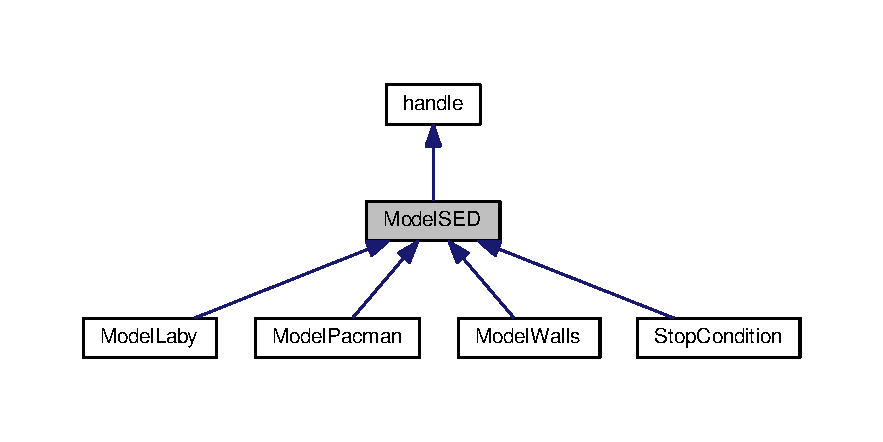
\includegraphics[width=350pt]{class_model_s_e_d__inherit__graph}
\end{center}
\end{figure}


Collaboration diagram for Model\+S\+ED\+:\nopagebreak
\begin{figure}[H]
\begin{center}
\leavevmode
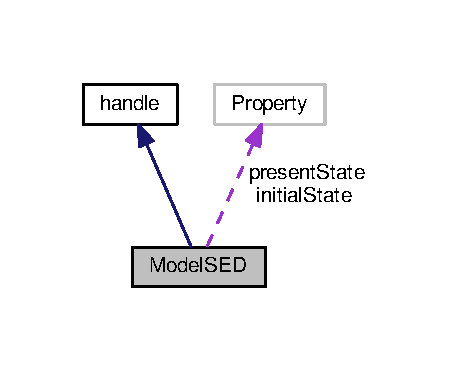
\includegraphics[width=216pt]{class_model_s_e_d__coll__graph}
\end{center}
\end{figure}
\subsection*{Public Member Functions}
\begin{DoxyCompactItemize}
\item 
virtual \hyperlink{class_model_s_e_d_ac36f9451c43b120828af4380858f2024}{f} (in obj, in in)
\begin{DoxyCompactList}\small\item\em Compute the evolution of the model. \end{DoxyCompactList}\item 
virtual \hyperlink{class_model_s_e_d_adb8aaccb857cf5bbec640cd00915459d}{m} (in obj, in next\+State, in init)
\begin{DoxyCompactList}\small\item\em Memory method update the state of the command. \end{DoxyCompactList}\item 
virtual \hyperlink{class_model_s_e_d_ac6bf71081e35755d5ed9992d165afcb8}{g} (in obj)
\begin{DoxyCompactList}\small\item\em Create the outputs. \end{DoxyCompactList}\end{DoxyCompactItemize}
\subsection*{Public Attributes}
\begin{DoxyCompactItemize}
\item 
Property \hyperlink{class_model_s_e_d_a9624cc7c421a50fa5086b0ebd0cd5fe3}{present\+State}
\begin{DoxyCompactList}\small\item\em This is the state of the command in the present moment. \end{DoxyCompactList}\item 
Property \hyperlink{class_model_s_e_d_acd9263acfa96c9138afdf497e55acc24}{initial\+State}
\begin{DoxyCompactList}\small\item\em This is the state of the command in the initialization and when it\textquotesingle{}s reseted. \end{DoxyCompactList}\end{DoxyCompactItemize}


\subsection{Detailed Description}
Abstract Class who contain the structure of a \char`\"{}fmg\char`\"{} implementation. 

This class is used for give a general definition of Model Class.~\newline
 Input \+: necessary information for compute the next state of the model ~\newline
~\newline
 Output \+: output\textquotesingle{}s action of the model~\newline
 State \+: minimal information necessary who evolute~\newline
 

\subsection{Member Function Documentation}
\mbox{\Hypertarget{class_model_s_e_d_ac36f9451c43b120828af4380858f2024}\label{class_model_s_e_d_ac36f9451c43b120828af4380858f2024}} 
\index{Model\+S\+ED@{Model\+S\+ED}!f@{f}}
\index{f@{f}!Model\+S\+ED@{Model\+S\+ED}}
\subsubsection{\texorpdfstring{f()}{f()}}
{\footnotesize\ttfamily virtual f (\begin{DoxyParamCaption}\item[{in}]{obj,  }\item[{in}]{in }\end{DoxyParamCaption})\hspace{0.3cm}{\ttfamily [virtual]}}



Compute the evolution of the model. 


\begin{DoxyParams}{Parameters}
{\em obj} & The instance who evolute \\
\hline
{\em in} & Input needed for the computing \\
\hline
\end{DoxyParams}

\begin{DoxyRetVals}{Return values}
{\em next\+State} & The future state of the model \\
\hline
\end{DoxyRetVals}


Reimplemented in \hyperlink{class_model_pacman_a6f3b146c92a207e95690d08975e1e072}{Model\+Pacman}, and \hyperlink{class_model_laby_a6f3b146c92a207e95690d08975e1e072}{Model\+Laby}.

\mbox{\Hypertarget{class_model_s_e_d_ac6bf71081e35755d5ed9992d165afcb8}\label{class_model_s_e_d_ac6bf71081e35755d5ed9992d165afcb8}} 
\index{Model\+S\+ED@{Model\+S\+ED}!g@{g}}
\index{g@{g}!Model\+S\+ED@{Model\+S\+ED}}
\subsubsection{\texorpdfstring{g()}{g()}}
{\footnotesize\ttfamily virtual g (\begin{DoxyParamCaption}\item[{in}]{obj }\end{DoxyParamCaption})\hspace{0.3cm}{\ttfamily [virtual]}}



Create the outputs. 


\begin{DoxyParams}{Parameters}
{\em obj} & the concerned instance of the class \\
\hline
\end{DoxyParams}

\begin{DoxyRetVals}{Return values}
{\em out} & Constructed output of the model \\
\hline
\end{DoxyRetVals}


Reimplemented in \hyperlink{class_model_ghost_a07dadfabe92bf9a144b8a862720e7746}{Model\+Ghost}, \hyperlink{class_model_laby_a07dadfabe92bf9a144b8a862720e7746}{Model\+Laby}, \hyperlink{class_model_pacman_a07dadfabe92bf9a144b8a862720e7746}{Model\+Pacman}, \hyperlink{class_stop_condition_a07dadfabe92bf9a144b8a862720e7746}{Stop\+Condition}, and \hyperlink{class_model_walls_a07dadfabe92bf9a144b8a862720e7746}{Model\+Walls}.

\mbox{\Hypertarget{class_model_s_e_d_adb8aaccb857cf5bbec640cd00915459d}\label{class_model_s_e_d_adb8aaccb857cf5bbec640cd00915459d}} 
\index{Model\+S\+ED@{Model\+S\+ED}!m@{m}}
\index{m@{m}!Model\+S\+ED@{Model\+S\+ED}}
\subsubsection{\texorpdfstring{m()}{m()}}
{\footnotesize\ttfamily virtual m (\begin{DoxyParamCaption}\item[{in}]{obj,  }\item[{in}]{next\+State,  }\item[{in}]{init }\end{DoxyParamCaption})\hspace{0.3cm}{\ttfamily [virtual]}}



Memory method update the state of the command. 


\begin{DoxyParams}{Parameters}
{\em obj} & The selected instance of the class \\
\hline
{\em next\+State} & The value of the state need to update \\
\hline
{\em init} & Boolean condition for initialize or reset the command \\
\hline
\end{DoxyParams}
\begin{DoxyReturn}{Returns}
instance of the class updated 
\end{DoxyReturn}


Reimplemented in \hyperlink{class_model_ghost_a3140f24c6c4b80037b7d4f521c6ae2d3}{Model\+Ghost}, \hyperlink{class_model_pacman_a3140f24c6c4b80037b7d4f521c6ae2d3}{Model\+Pacman}, \hyperlink{class_model_laby_a3140f24c6c4b80037b7d4f521c6ae2d3}{Model\+Laby}, \hyperlink{class_stop_condition_a3140f24c6c4b80037b7d4f521c6ae2d3}{Stop\+Condition}, and \hyperlink{class_model_walls_a3140f24c6c4b80037b7d4f521c6ae2d3}{Model\+Walls}.



\subsection{Member Data Documentation}
\mbox{\Hypertarget{class_model_s_e_d_acd9263acfa96c9138afdf497e55acc24}\label{class_model_s_e_d_acd9263acfa96c9138afdf497e55acc24}} 
\index{Model\+S\+ED@{Model\+S\+ED}!initial\+State@{initial\+State}}
\index{initial\+State@{initial\+State}!Model\+S\+ED@{Model\+S\+ED}}
\subsubsection{\texorpdfstring{initial\+State}{initialState}}
{\footnotesize\ttfamily Property initial\+State}



This is the state of the command in the initialization and when it\textquotesingle{}s reseted. 

\mbox{\Hypertarget{class_model_s_e_d_a9624cc7c421a50fa5086b0ebd0cd5fe3}\label{class_model_s_e_d_a9624cc7c421a50fa5086b0ebd0cd5fe3}} 
\index{Model\+S\+ED@{Model\+S\+ED}!present\+State@{present\+State}}
\index{present\+State@{present\+State}!Model\+S\+ED@{Model\+S\+ED}}
\subsubsection{\texorpdfstring{present\+State}{presentState}}
{\footnotesize\ttfamily Property present\+State}



This is the state of the command in the present moment. 



The documentation for this class was generated from the following file\+:\begin{DoxyCompactItemize}
\item 
\hyperlink{_model_s_e_d_8m}{Model\+S\+E\+D.\+m}\end{DoxyCompactItemize}

\hypertarget{class_model_walls}{}\section{Model\+Walls Class Reference}
\label{class_model_walls}\index{Model\+Walls@{Model\+Walls}}


Contain wall movement command.  




Inheritance diagram for Model\+Walls\+:\nopagebreak
\begin{figure}[H]
\begin{center}
\leavevmode
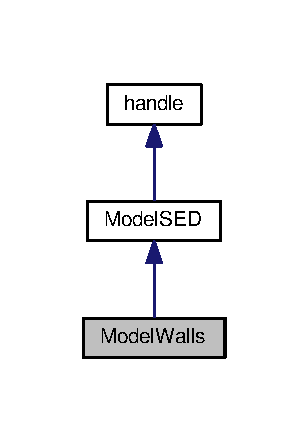
\includegraphics[width=148pt]{class_model_walls__inherit__graph}
\end{center}
\end{figure}


Collaboration diagram for Model\+Walls\+:\nopagebreak
\begin{figure}[H]
\begin{center}
\leavevmode
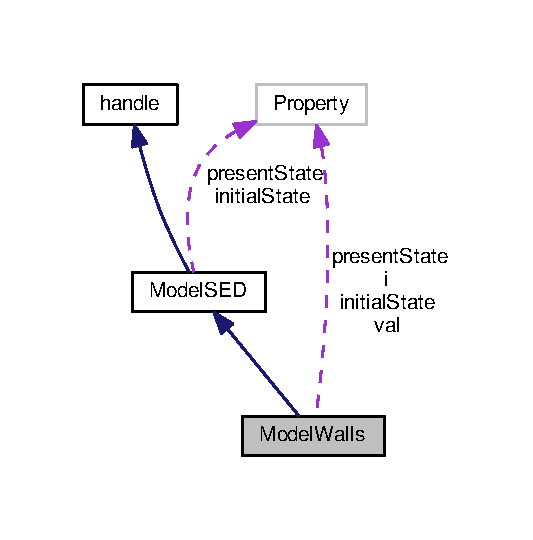
\includegraphics[width=256pt]{class_model_walls__coll__graph}
\end{center}
\end{figure}
\subsection*{Public Member Functions}
\begin{DoxyCompactItemize}
\item 
function \hyperlink{class_model_walls_a5aa5cfd2186c06e8ab37ce531b1a9720}{Model\+Walls} (in init\+Value)
\begin{DoxyCompactList}\small\item\em Class constructor. \end{DoxyCompactList}\item 
function \hyperlink{class_model_walls_af07620c51528eb1e504befcf52ca0cee}{f} (in obj)
\item 
function \hyperlink{class_model_walls_a3140f24c6c4b80037b7d4f521c6ae2d3}{m} (in obj, in next\+State, in init)
\begin{DoxyCompactList}\small\item\em Memory method update the state of the command. \end{DoxyCompactList}\item 
function \hyperlink{class_model_walls_a07dadfabe92bf9a144b8a862720e7746}{g} (in obj)
\begin{DoxyCompactList}\small\item\em Create the outputs. \end{DoxyCompactList}\item 
virtual \hyperlink{class_model_s_e_d_ac36f9451c43b120828af4380858f2024}{f} (in obj, in in)
\begin{DoxyCompactList}\small\item\em Compute the evolution of the model. \end{DoxyCompactList}\end{DoxyCompactItemize}
\subsection*{Public Attributes}
\begin{DoxyCompactItemize}
\item 
Property \hyperlink{class_model_walls_a9624cc7c421a50fa5086b0ebd0cd5fe3}{present\+State}
\item 
Property \hyperlink{class_model_walls_acd9263acfa96c9138afdf497e55acc24}{initial\+State}
\item 
Property \hyperlink{class_model_walls_a103c618d75e54c3a72fac6bcaa59f61f}{i}
\item 
Property \hyperlink{class_model_walls_aae3a423b8c844683e2adba0472347fe1}{val}
\end{DoxyCompactItemize}


\subsection{Detailed Description}
Contain wall movement command. 

Input \+: No need ~\newline
 ~\newline
 Output \+: \mbox{[}U\+Pwalls , R\+I\+G\+H\+Twalls\mbox{]}~\newline
 ~\newline
 State \+: contain the last move ( 0 = up ; 1 = right) ~\newline
 This command do the sequence walls Right --$>$ walls down ~\newline
 

\subsection{Constructor \& Destructor Documentation}
\mbox{\Hypertarget{class_model_walls_a5aa5cfd2186c06e8ab37ce531b1a9720}\label{class_model_walls_a5aa5cfd2186c06e8ab37ce531b1a9720}} 
\index{Model\+Walls@{Model\+Walls}!Model\+Walls@{Model\+Walls}}
\index{Model\+Walls@{Model\+Walls}!Model\+Walls@{Model\+Walls}}
\subsubsection{\texorpdfstring{Model\+Walls()}{ModelWalls()}}
{\footnotesize\ttfamily function \hyperlink{class_model_walls}{Model\+Walls} (\begin{DoxyParamCaption}\item[{in}]{init\+Value }\end{DoxyParamCaption})}



Class constructor. 


\begin{DoxyParams}{Parameters}
{\em initial\+Value} & Contain the initial state \\
\hline
\end{DoxyParams}
\begin{DoxyReturn}{Returns}
instance of the \hyperlink{class_model_walls}{Model\+Walls} class. 
\end{DoxyReturn}


\subsection{Member Function Documentation}
\mbox{\Hypertarget{class_model_s_e_d_ac36f9451c43b120828af4380858f2024}\label{class_model_s_e_d_ac36f9451c43b120828af4380858f2024}} 
\index{Model\+Walls@{Model\+Walls}!f@{f}}
\index{f@{f}!Model\+Walls@{Model\+Walls}}
\subsubsection{\texorpdfstring{f()}{f()}\hspace{0.1cm}{\footnotesize\ttfamily [1/2]}}
{\footnotesize\ttfamily virtual f (\begin{DoxyParamCaption}\item[{in}]{obj,  }\item[{in}]{in }\end{DoxyParamCaption})\hspace{0.3cm}{\ttfamily [virtual]}, {\ttfamily [inherited]}}



Compute the evolution of the model. 


\begin{DoxyParams}{Parameters}
{\em obj} & The instance who evolute \\
\hline
{\em in} & Input needed for the computing \\
\hline
\end{DoxyParams}

\begin{DoxyRetVals}{Return values}
{\em next\+State} & The future state of the model \\
\hline
\end{DoxyRetVals}


Reimplemented in \hyperlink{class_model_pacman_a6f3b146c92a207e95690d08975e1e072}{Model\+Pacman}, and \hyperlink{class_model_laby_a6f3b146c92a207e95690d08975e1e072}{Model\+Laby}.

\mbox{\Hypertarget{class_model_walls_af07620c51528eb1e504befcf52ca0cee}\label{class_model_walls_af07620c51528eb1e504befcf52ca0cee}} 
\index{Model\+Walls@{Model\+Walls}!f@{f}}
\index{f@{f}!Model\+Walls@{Model\+Walls}}
\subsubsection{\texorpdfstring{f()}{f()}\hspace{0.1cm}{\footnotesize\ttfamily [2/2]}}
{\footnotesize\ttfamily function f (\begin{DoxyParamCaption}\item[{in}]{obj }\end{DoxyParamCaption})}

\mbox{\Hypertarget{class_model_walls_a07dadfabe92bf9a144b8a862720e7746}\label{class_model_walls_a07dadfabe92bf9a144b8a862720e7746}} 
\index{Model\+Walls@{Model\+Walls}!g@{g}}
\index{g@{g}!Model\+Walls@{Model\+Walls}}
\subsubsection{\texorpdfstring{g()}{g()}}
{\footnotesize\ttfamily function g (\begin{DoxyParamCaption}\item[{in}]{obj }\end{DoxyParamCaption})\hspace{0.3cm}{\ttfamily [virtual]}}



Create the outputs. 


\begin{DoxyParams}{Parameters}
{\em obj} & the concerned instance of the class \\
\hline
\end{DoxyParams}

\begin{DoxyRetVals}{Return values}
{\em out} & The output who is the command. \\
\hline
\end{DoxyRetVals}


Reimplemented from \hyperlink{class_model_s_e_d_ac6bf71081e35755d5ed9992d165afcb8}{Model\+S\+ED}.

\mbox{\Hypertarget{class_model_walls_a3140f24c6c4b80037b7d4f521c6ae2d3}\label{class_model_walls_a3140f24c6c4b80037b7d4f521c6ae2d3}} 
\index{Model\+Walls@{Model\+Walls}!m@{m}}
\index{m@{m}!Model\+Walls@{Model\+Walls}}
\subsubsection{\texorpdfstring{m()}{m()}}
{\footnotesize\ttfamily function m (\begin{DoxyParamCaption}\item[{in}]{obj,  }\item[{in}]{next\+State,  }\item[{in}]{init }\end{DoxyParamCaption})\hspace{0.3cm}{\ttfamily [virtual]}}



Memory method update the state of the command. 


\begin{DoxyParams}{Parameters}
{\em obj} & The selected instance of the class \\
\hline
{\em next\+State} & The value of the state need to update \\
\hline
{\em init} & Boolean condition for initialize or reset the command \\
\hline
\end{DoxyParams}
\begin{DoxyReturn}{Returns}
instance of the class updated 
\end{DoxyReturn}


Reimplemented from \hyperlink{class_model_s_e_d_adb8aaccb857cf5bbec640cd00915459d}{Model\+S\+ED}.



\subsection{Member Data Documentation}
\mbox{\Hypertarget{class_model_walls_a103c618d75e54c3a72fac6bcaa59f61f}\label{class_model_walls_a103c618d75e54c3a72fac6bcaa59f61f}} 
\index{Model\+Walls@{Model\+Walls}!i@{i}}
\index{i@{i}!Model\+Walls@{Model\+Walls}}
\subsubsection{\texorpdfstring{i}{i}}
{\footnotesize\ttfamily Property i}

\mbox{\Hypertarget{class_model_walls_acd9263acfa96c9138afdf497e55acc24}\label{class_model_walls_acd9263acfa96c9138afdf497e55acc24}} 
\index{Model\+Walls@{Model\+Walls}!initial\+State@{initial\+State}}
\index{initial\+State@{initial\+State}!Model\+Walls@{Model\+Walls}}
\subsubsection{\texorpdfstring{initial\+State}{initialState}}
{\footnotesize\ttfamily Property initial\+State}

\mbox{\Hypertarget{class_model_walls_a9624cc7c421a50fa5086b0ebd0cd5fe3}\label{class_model_walls_a9624cc7c421a50fa5086b0ebd0cd5fe3}} 
\index{Model\+Walls@{Model\+Walls}!present\+State@{present\+State}}
\index{present\+State@{present\+State}!Model\+Walls@{Model\+Walls}}
\subsubsection{\texorpdfstring{present\+State}{presentState}}
{\footnotesize\ttfamily Property present\+State}

\mbox{\Hypertarget{class_model_walls_aae3a423b8c844683e2adba0472347fe1}\label{class_model_walls_aae3a423b8c844683e2adba0472347fe1}} 
\index{Model\+Walls@{Model\+Walls}!val@{val}}
\index{val@{val}!Model\+Walls@{Model\+Walls}}
\subsubsection{\texorpdfstring{val}{val}}
{\footnotesize\ttfamily Property val}



The documentation for this class was generated from the following file\+:\begin{DoxyCompactItemize}
\item 
\hyperlink{_model_walls_8m}{Model\+Walls.\+m}\end{DoxyCompactItemize}

\hypertarget{class_stop_condition}{}\section{Stop\+Condition Class Reference}
\label{class_stop_condition}\index{Stop\+Condition@{Stop\+Condition}}


Inheritance diagram for Stop\+Condition\+:
\nopagebreak
\begin{figure}[H]
\begin{center}
\leavevmode
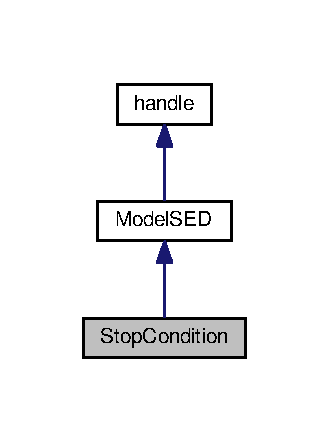
\includegraphics[width=158pt]{class_stop_condition__inherit__graph}
\end{center}
\end{figure}


Collaboration diagram for Stop\+Condition\+:
\nopagebreak
\begin{figure}[H]
\begin{center}
\leavevmode
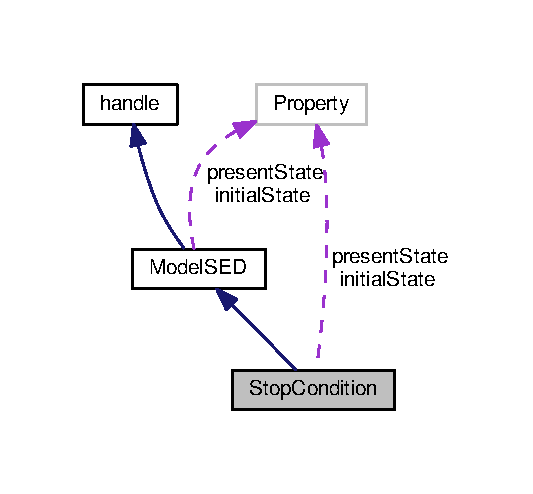
\includegraphics[width=256pt]{class_stop_condition__coll__graph}
\end{center}
\end{figure}
\subsection*{Public Member Functions}
\begin{DoxyCompactItemize}
\item 
\hyperlink{_plan__desuma_functions_8m_ac2ffb26d6f42d3bbcd7847b0873403f4}{function} \hyperlink{class_stop_condition_a998151731b2f85cb0f3e0cbc7d82bf96}{Stop\+Condition} (in init\+Condition)
\item 
\hyperlink{_plan__desuma_functions_8m_ac2ffb26d6f42d3bbcd7847b0873403f4}{function} \hyperlink{class_stop_condition_abcffcbb16870f569058af2fd7823c5dd}{f} (in obj, in no\+Escape, in pacman\+Walls\+Break)
\item 
\hyperlink{_plan__desuma_functions_8m_ac2ffb26d6f42d3bbcd7847b0873403f4}{function} \hyperlink{class_stop_condition_a3140f24c6c4b80037b7d4f521c6ae2d3}{m} (in obj, in next\+State, in init)
\begin{DoxyCompactList}\small\item\em Memory method update the state of the command. \end{DoxyCompactList}\item 
\hyperlink{_plan__desuma_functions_8m_ac2ffb26d6f42d3bbcd7847b0873403f4}{function} \hyperlink{class_stop_condition_a07dadfabe92bf9a144b8a862720e7746}{g} (in obj)
\begin{DoxyCompactList}\small\item\em Create the outputs. \end{DoxyCompactList}\item 
virtual \hyperlink{class_model_s_e_d_ac36f9451c43b120828af4380858f2024}{f} (in obj, in in)
\begin{DoxyCompactList}\small\item\em Compute the evolution of the model. \end{DoxyCompactList}\end{DoxyCompactItemize}
\subsection*{Public Attributes}
\begin{DoxyCompactItemize}
\item 
Property \hyperlink{class_stop_condition_a9624cc7c421a50fa5086b0ebd0cd5fe3}{present\+State}
\item 
Property \hyperlink{class_stop_condition_acd9263acfa96c9138afdf497e55acc24}{initial\+State}
\end{DoxyCompactItemize}


\subsection{Constructor \& Destructor Documentation}
\mbox{\Hypertarget{class_stop_condition_a998151731b2f85cb0f3e0cbc7d82bf96}\label{class_stop_condition_a998151731b2f85cb0f3e0cbc7d82bf96}} 
\index{Stop\+Condition@{Stop\+Condition}!Stop\+Condition@{Stop\+Condition}}
\index{Stop\+Condition@{Stop\+Condition}!Stop\+Condition@{Stop\+Condition}}
\subsubsection{\texorpdfstring{Stop\+Condition()}{StopCondition()}}
{\footnotesize\ttfamily \hyperlink{_plan__desuma_functions_8m_ac2ffb26d6f42d3bbcd7847b0873403f4}{function} \hyperlink{class_stop_condition}{Stop\+Condition} (\begin{DoxyParamCaption}\item[{in}]{init\+Condition }\end{DoxyParamCaption})}



\subsection{Member Function Documentation}
\mbox{\Hypertarget{class_stop_condition_abcffcbb16870f569058af2fd7823c5dd}\label{class_stop_condition_abcffcbb16870f569058af2fd7823c5dd}} 
\index{Stop\+Condition@{Stop\+Condition}!f@{f}}
\index{f@{f}!Stop\+Condition@{Stop\+Condition}}
\subsubsection{\texorpdfstring{f()}{f()}\hspace{0.1cm}{\footnotesize\ttfamily [1/2]}}
{\footnotesize\ttfamily \hyperlink{_plan__desuma_functions_8m_ac2ffb26d6f42d3bbcd7847b0873403f4}{function} f (\begin{DoxyParamCaption}\item[{in}]{obj,  }\item[{in}]{no\+Escape,  }\item[{in}]{pacman\+Walls\+Break }\end{DoxyParamCaption})}

\mbox{\Hypertarget{class_model_s_e_d_ac36f9451c43b120828af4380858f2024}\label{class_model_s_e_d_ac36f9451c43b120828af4380858f2024}} 
\index{Stop\+Condition@{Stop\+Condition}!f@{f}}
\index{f@{f}!Stop\+Condition@{Stop\+Condition}}
\subsubsection{\texorpdfstring{f()}{f()}\hspace{0.1cm}{\footnotesize\ttfamily [2/2]}}
{\footnotesize\ttfamily virtual f (\begin{DoxyParamCaption}\item[{in}]{obj,  }\item[{in}]{in }\end{DoxyParamCaption})\hspace{0.3cm}{\ttfamily [virtual]}, {\ttfamily [inherited]}}



Compute the evolution of the model. 


\begin{DoxyParams}{Parameters}
{\em obj} & The instance who evolute \\
\hline
{\em in} & Input needed for the computing \\
\hline
\end{DoxyParams}

\begin{DoxyRetVals}{Return values}
{\em next\+State} & The future state of the model \\
\hline
\end{DoxyRetVals}


Reimplemented in \hyperlink{class_model_pacman_a6f3b146c92a207e95690d08975e1e072}{Model\+Pacman}, and \hyperlink{class_model_laby_a6f3b146c92a207e95690d08975e1e072}{Model\+Laby}.

\mbox{\Hypertarget{class_stop_condition_a07dadfabe92bf9a144b8a862720e7746}\label{class_stop_condition_a07dadfabe92bf9a144b8a862720e7746}} 
\index{Stop\+Condition@{Stop\+Condition}!g@{g}}
\index{g@{g}!Stop\+Condition@{Stop\+Condition}}
\subsubsection{\texorpdfstring{g()}{g()}}
{\footnotesize\ttfamily \hyperlink{_plan__desuma_functions_8m_ac2ffb26d6f42d3bbcd7847b0873403f4}{function} g (\begin{DoxyParamCaption}\item[{in}]{obj }\end{DoxyParamCaption})\hspace{0.3cm}{\ttfamily [virtual]}}



Create the outputs. 


\begin{DoxyParams}{Parameters}
{\em obj} & the concerned instance of the class \\
\hline
\end{DoxyParams}

\begin{DoxyRetVals}{Return values}
{\em out} & Constructed output of the model \\
\hline
\end{DoxyRetVals}


Reimplemented from \hyperlink{class_model_s_e_d_ac6bf71081e35755d5ed9992d165afcb8}{Model\+S\+ED}.

\mbox{\Hypertarget{class_stop_condition_a3140f24c6c4b80037b7d4f521c6ae2d3}\label{class_stop_condition_a3140f24c6c4b80037b7d4f521c6ae2d3}} 
\index{Stop\+Condition@{Stop\+Condition}!m@{m}}
\index{m@{m}!Stop\+Condition@{Stop\+Condition}}
\subsubsection{\texorpdfstring{m()}{m()}}
{\footnotesize\ttfamily \hyperlink{_plan__desuma_functions_8m_ac2ffb26d6f42d3bbcd7847b0873403f4}{function} m (\begin{DoxyParamCaption}\item[{in}]{obj,  }\item[{in}]{next\+State,  }\item[{in}]{init }\end{DoxyParamCaption})\hspace{0.3cm}{\ttfamily [virtual]}}



Memory method update the state of the command. 


\begin{DoxyParams}{Parameters}
{\em obj} & The selected instance of the class \\
\hline
{\em next\+State} & The value of the state need to update \\
\hline
{\em init} & Boolean condition for initialize or reset the command \\
\hline
\end{DoxyParams}
\begin{DoxyReturn}{Returns}
instance of the class updated 
\end{DoxyReturn}


Reimplemented from \hyperlink{class_model_s_e_d_adb8aaccb857cf5bbec640cd00915459d}{Model\+S\+ED}.



\subsection{Member Data Documentation}
\mbox{\Hypertarget{class_stop_condition_acd9263acfa96c9138afdf497e55acc24}\label{class_stop_condition_acd9263acfa96c9138afdf497e55acc24}} 
\index{Stop\+Condition@{Stop\+Condition}!initial\+State@{initial\+State}}
\index{initial\+State@{initial\+State}!Stop\+Condition@{Stop\+Condition}}
\subsubsection{\texorpdfstring{initial\+State}{initialState}}
{\footnotesize\ttfamily Property initial\+State}

\mbox{\Hypertarget{class_stop_condition_a9624cc7c421a50fa5086b0ebd0cd5fe3}\label{class_stop_condition_a9624cc7c421a50fa5086b0ebd0cd5fe3}} 
\index{Stop\+Condition@{Stop\+Condition}!present\+State@{present\+State}}
\index{present\+State@{present\+State}!Stop\+Condition@{Stop\+Condition}}
\subsubsection{\texorpdfstring{present\+State}{presentState}}
{\footnotesize\ttfamily Property present\+State}



The documentation for this class was generated from the following file\+:\begin{DoxyCompactItemize}
\item 
\hyperlink{_stop_condition_8m}{Stop\+Condition.\+m}\end{DoxyCompactItemize}

\hypertarget{class_wrapper}{}\section{Wrapper Class Reference}
\label{class_wrapper}\index{Wrapper@{Wrapper}}


Connects all models to the display function.  




Collaboration diagram for Wrapper\+:\nopagebreak
\begin{figure}[H]
\begin{center}
\leavevmode
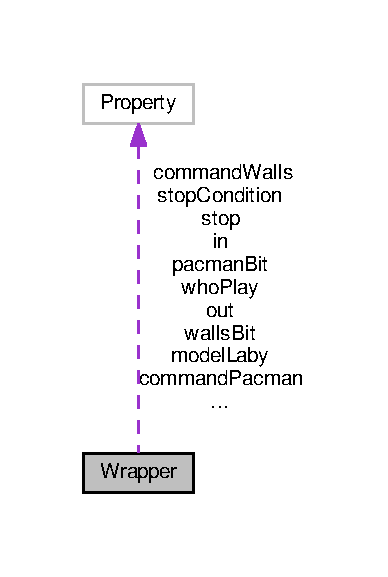
\includegraphics[width=186pt]{class_wrapper__coll__graph}
\end{center}
\end{figure}
\subsection*{Public Member Functions}
\begin{DoxyCompactItemize}
\item 
function \hyperlink{class_wrapper_ab0ebf6c7738beb446d13d2d9445fbc8a}{Wrapper} (\hyperlink{class_wrapper_a5e252d97ca5bf85c5753e2914673eead}{in} in\+Size, \hyperlink{class_wrapper_a5e252d97ca5bf85c5753e2914673eead}{in} out\+Size, \hyperlink{class_wrapper_a5e252d97ca5bf85c5753e2914673eead}{in} init\+Laby, \hyperlink{class_wrapper_a5e252d97ca5bf85c5753e2914673eead}{in} init\+Walls, \hyperlink{class_wrapper_a5e252d97ca5bf85c5753e2914673eead}{in} init\+Pac, \hyperlink{class_wrapper_a5e252d97ca5bf85c5753e2914673eead}{in} init\+Stop)
\begin{DoxyCompactList}\small\item\em Class constructor of Instance of \hyperlink{class_stop_condition}{Stop\+Condition} Class. \end{DoxyCompactList}\item 
function \hyperlink{class_wrapper_aa41b9b215897635f48e1c8a4eaca7640}{update\+Connexion} (\hyperlink{class_wrapper_a5e252d97ca5bf85c5753e2914673eead}{in} obj, \hyperlink{class_wrapper_a5e252d97ca5bf85c5753e2914673eead}{in} ind\+Bit, \hyperlink{class_wrapper_a5e252d97ca5bf85c5753e2914673eead}{in} value)
\begin{DoxyCompactList}\small\item\em Update the connection bit for connect automatic mode for Pacman and/or the walls. \end{DoxyCompactList}\item 
function \hyperlink{class_wrapper_a7d486dd79e7c7bc857ffaa4e273d27c5}{init} (\hyperlink{class_wrapper_a5e252d97ca5bf85c5753e2914673eead}{in} obj)
\begin{DoxyCompactList}\small\item\em Allows to completely reset the labyrinth. \end{DoxyCompactList}\item 
function \hyperlink{class_wrapper_a9c889c73b9d4b80dde64dfe385ed747e}{orderer} (\hyperlink{class_wrapper_a5e252d97ca5bf85c5753e2914673eead}{in} obj, \hyperlink{class_wrapper_a5e252d97ca5bf85c5753e2914673eead}{in} vect\+In)
\begin{DoxyCompactList}\small\item\em Ordinate the global execution of Models. \end{DoxyCompactList}\item 
function \hyperlink{class_wrapper_aaba4a98b8b3bf391348722f0f227e333}{get\+\_\+stop} (\hyperlink{class_wrapper_a5e252d97ca5bf85c5753e2914673eead}{in} obj)
\begin{DoxyCompactList}\small\item\em Return the current State of shutdown condition. \end{DoxyCompactList}\item 
function \hyperlink{class_wrapper_a15af7c208437e3c98d1f130b45a36a37}{get\+\_\+out} (\hyperlink{class_wrapper_a5e252d97ca5bf85c5753e2914673eead}{in} obj)
\begin{DoxyCompactList}\small\item\em Return the current State of output cell. \end{DoxyCompactList}\end{DoxyCompactItemize}
\subsection*{Public Attributes}
\begin{DoxyCompactItemize}
\item 
Property \hyperlink{class_wrapper_a94dd71be012b98d496117309a20939b1}{walls\+Bit}
\begin{DoxyCompactList}\small\item\em Boolean connection for the walls. \end{DoxyCompactList}\item 
Property \hyperlink{class_wrapper_abf190bfcb1e7ec7573c4e002d30cb125}{pacman\+Bit}
\begin{DoxyCompactList}\small\item\em Boolean connection for the Pacman. \end{DoxyCompactList}\item 
Property \hyperlink{class_wrapper_a65b2390d6d3e36b42ee0ea886a562d5c}{model\+Laby}
\begin{DoxyCompactList}\small\item\em contain the instance of the model of labyrinth. \end{DoxyCompactList}\item 
Property \hyperlink{class_wrapper_ae0183c9714a832124ccb420d5f9d3c1f}{command\+Walls}
\begin{DoxyCompactList}\small\item\em contain the instance of wall\textquotesingle{}s command. \end{DoxyCompactList}\item 
Property \hyperlink{class_wrapper_ab39f6156efa48a09b1d92e22eb9fc94a}{command\+Pacman}
\begin{DoxyCompactList}\small\item\em contain the instance of Pacman\textquotesingle{}s command. \end{DoxyCompactList}\item 
Property \hyperlink{class_wrapper_a19a246dc459b20945f02106d6734fa4b}{stop\+Condition}
\begin{DoxyCompactList}\small\item\em contain the instance shutdown condition. \end{DoxyCompactList}\item 
Property \hyperlink{class_wrapper_a5e252d97ca5bf85c5753e2914673eead}{in}
\begin{DoxyCompactList}\small\item\em A integer vector who contain the state of input,. \end{DoxyCompactList}\item 
Property \hyperlink{class_wrapper_a8fcb5c64317d463be34f501200a2f49a}{out}
\begin{DoxyCompactList}\small\item\em A cell who contain the state of output,. \end{DoxyCompactList}\item 
Property \hyperlink{class_wrapper_ab453e11b3a41f7ef03be604bb5182e76}{stop}
\begin{DoxyCompactList}\small\item\em A cell that contains the output of the stop conditions instance. \end{DoxyCompactList}\item 
Property \hyperlink{class_wrapper_a19e8c1d68257003eba8e5a47c8302113}{who\+Play}
\begin{DoxyCompactList}\small\item\em A increment integer that permit to know which object to play 0 = walls ; 1 = Pacman. \end{DoxyCompactList}\end{DoxyCompactItemize}


\subsection{Detailed Description}
Connects all models to the display function. 

Contain the connection between the different elements and contain all the models (walls, labyrinth, Pacman, escape) 

\subsection{Constructor \& Destructor Documentation}
\mbox{\Hypertarget{class_wrapper_ab0ebf6c7738beb446d13d2d9445fbc8a}\label{class_wrapper_ab0ebf6c7738beb446d13d2d9445fbc8a}} 
\index{Wrapper@{Wrapper}!Wrapper@{Wrapper}}
\index{Wrapper@{Wrapper}!Wrapper@{Wrapper}}
\subsubsection{\texorpdfstring{Wrapper()}{Wrapper()}}
{\footnotesize\ttfamily function \hyperlink{class_wrapper}{Wrapper} (\begin{DoxyParamCaption}\item[{\hyperlink{class_wrapper_a5e252d97ca5bf85c5753e2914673eead}{in}}]{in\+Size,  }\item[{\hyperlink{class_wrapper_a5e252d97ca5bf85c5753e2914673eead}{in}}]{out\+Size,  }\item[{\hyperlink{class_wrapper_a5e252d97ca5bf85c5753e2914673eead}{in}}]{init\+Laby,  }\item[{\hyperlink{class_wrapper_a5e252d97ca5bf85c5753e2914673eead}{in}}]{init\+Walls,  }\item[{\hyperlink{class_wrapper_a5e252d97ca5bf85c5753e2914673eead}{in}}]{init\+Pac,  }\item[{\hyperlink{class_wrapper_a5e252d97ca5bf85c5753e2914673eead}{in}}]{init\+Stop }\end{DoxyParamCaption})}



Class constructor of Instance of \hyperlink{class_stop_condition}{Stop\+Condition} Class. 


\begin{DoxyParams}{Parameters}
{\em in\+Size} & Integer containing the size of the state of inputs. \\
\hline
{\em out\+Size} & Integer containing the size of the state of Outputs. \\
\hline
{\em init\+Laby} & Structure containing every fields need to initialize the labyrinth Model. \\
\hline
{\em init\+Walls} & Structure containing every fields need to initialize the Walls Model. \\
\hline
{\em init\+Pac} & Structure containing every fields need to initialize the Pacman Model. \\
\hline
{\em init\+Stop} & Structure containing every fields need to initialize the Stop Model. \\
\hline
\end{DoxyParams}
\begin{DoxyReturn}{Returns}
instance of the \hyperlink{class_wrapper}{Wrapper} class. 
\end{DoxyReturn}


\subsection{Member Function Documentation}
\mbox{\Hypertarget{class_wrapper_a15af7c208437e3c98d1f130b45a36a37}\label{class_wrapper_a15af7c208437e3c98d1f130b45a36a37}} 
\index{Wrapper@{Wrapper}!get\+\_\+out@{get\+\_\+out}}
\index{get\+\_\+out@{get\+\_\+out}!Wrapper@{Wrapper}}
\subsubsection{\texorpdfstring{get\+\_\+out()}{get\_out()}}
{\footnotesize\ttfamily function get\+\_\+out (\begin{DoxyParamCaption}\item[{\hyperlink{class_wrapper_a5e252d97ca5bf85c5753e2914673eead}{in}}]{obj }\end{DoxyParamCaption})}



Return the current State of output cell. 


\begin{DoxyParams}{Parameters}
{\em obj} & The instance of \hyperlink{class_wrapper}{Wrapper}. \\
\hline
\end{DoxyParams}
\begin{DoxyReturn}{Returns}
Output cell. 
\end{DoxyReturn}
\mbox{\Hypertarget{class_wrapper_aaba4a98b8b3bf391348722f0f227e333}\label{class_wrapper_aaba4a98b8b3bf391348722f0f227e333}} 
\index{Wrapper@{Wrapper}!get\+\_\+stop@{get\+\_\+stop}}
\index{get\+\_\+stop@{get\+\_\+stop}!Wrapper@{Wrapper}}
\subsubsection{\texorpdfstring{get\+\_\+stop()}{get\_stop()}}
{\footnotesize\ttfamily function get\+\_\+stop (\begin{DoxyParamCaption}\item[{\hyperlink{class_wrapper_a5e252d97ca5bf85c5753e2914673eead}{in}}]{obj }\end{DoxyParamCaption})}



Return the current State of shutdown condition. 


\begin{DoxyParams}{Parameters}
{\em obj} & The instance of \hyperlink{class_wrapper}{Wrapper}. \\
\hline
\end{DoxyParams}
\begin{DoxyReturn}{Returns}
instance of the Stop class. 
\end{DoxyReturn}
\mbox{\Hypertarget{class_wrapper_a7d486dd79e7c7bc857ffaa4e273d27c5}\label{class_wrapper_a7d486dd79e7c7bc857ffaa4e273d27c5}} 
\index{Wrapper@{Wrapper}!init@{init}}
\index{init@{init}!Wrapper@{Wrapper}}
\subsubsection{\texorpdfstring{init()}{init()}}
{\footnotesize\ttfamily function init (\begin{DoxyParamCaption}\item[{\hyperlink{class_wrapper_a5e252d97ca5bf85c5753e2914673eead}{in}}]{obj }\end{DoxyParamCaption})}



Allows to completely reset the labyrinth. 


\begin{DoxyParams}{Parameters}
{\em obj} & The instance of \hyperlink{class_wrapper}{Wrapper}. \\
\hline
\end{DoxyParams}
\begin{DoxyReturn}{Returns}
instance of the \hyperlink{class_wrapper}{Wrapper} class. 
\end{DoxyReturn}
\mbox{\Hypertarget{class_wrapper_a9c889c73b9d4b80dde64dfe385ed747e}\label{class_wrapper_a9c889c73b9d4b80dde64dfe385ed747e}} 
\index{Wrapper@{Wrapper}!orderer@{orderer}}
\index{orderer@{orderer}!Wrapper@{Wrapper}}
\subsubsection{\texorpdfstring{orderer()}{orderer()}}
{\footnotesize\ttfamily function orderer (\begin{DoxyParamCaption}\item[{\hyperlink{class_wrapper_a5e252d97ca5bf85c5753e2914673eead}{in}}]{obj,  }\item[{\hyperlink{class_wrapper_a5e252d97ca5bf85c5753e2914673eead}{in}}]{vect\+In }\end{DoxyParamCaption})}



Ordinate the global execution of Models. 


\begin{DoxyParams}{Parameters}
{\em obj} & The instance of \hyperlink{class_wrapper}{Wrapper}. \\
\hline
\end{DoxyParams}
\begin{DoxyReturn}{Returns}
instance of the \hyperlink{class_wrapper}{Wrapper} class. In a first case, it checks which models is connected via the interface. If a model is connected, we execute the \textquotesingle{}fmg\textquotesingle{} structure of the model, else, we are waiting that a player push the desired button to move the labyrinth.~\newline
~\newline
 Here a little graphic about the scheduling of the call of each model \+: walls $>$ Laby $>$ pacman $>$ laby ~\newline
 Every call of \textquotesingle{}laby\textquotesingle{} implies a call of Stop Condition. 
\end{DoxyReturn}
\mbox{\Hypertarget{class_wrapper_aa41b9b215897635f48e1c8a4eaca7640}\label{class_wrapper_aa41b9b215897635f48e1c8a4eaca7640}} 
\index{Wrapper@{Wrapper}!update\+Connexion@{update\+Connexion}}
\index{update\+Connexion@{update\+Connexion}!Wrapper@{Wrapper}}
\subsubsection{\texorpdfstring{update\+Connexion()}{updateConnexion()}}
{\footnotesize\ttfamily function update\+Connexion (\begin{DoxyParamCaption}\item[{\hyperlink{class_wrapper_a5e252d97ca5bf85c5753e2914673eead}{in}}]{obj,  }\item[{\hyperlink{class_wrapper_a5e252d97ca5bf85c5753e2914673eead}{in}}]{ind\+Bit,  }\item[{\hyperlink{class_wrapper_a5e252d97ca5bf85c5753e2914673eead}{in}}]{value }\end{DoxyParamCaption})}



Update the connection bit for connect automatic mode for Pacman and/or the walls. 


\begin{DoxyParams}{Parameters}
{\em obj} & The instance of \hyperlink{class_wrapper}{Wrapper}. \\
\hline
{\em ind\+Bit} & Integer pointing the element to be connected \+: \textquotesingle{}1\textquotesingle{} for walls and \textquotesingle{}3\textquotesingle{} for Pacman. \\
\hline
{\em value} & Boolean indicating if the element is connected (True) or not. \\
\hline
\end{DoxyParams}
\begin{DoxyReturn}{Returns}
instance of the \hyperlink{class_wrapper}{Wrapper} class. 
\end{DoxyReturn}


\subsection{Member Data Documentation}
\mbox{\Hypertarget{class_wrapper_ab39f6156efa48a09b1d92e22eb9fc94a}\label{class_wrapper_ab39f6156efa48a09b1d92e22eb9fc94a}} 
\index{Wrapper@{Wrapper}!command\+Pacman@{command\+Pacman}}
\index{command\+Pacman@{command\+Pacman}!Wrapper@{Wrapper}}
\subsubsection{\texorpdfstring{command\+Pacman}{commandPacman}}
{\footnotesize\ttfamily Property command\+Pacman}



contain the instance of Pacman\textquotesingle{}s command. 

\mbox{\Hypertarget{class_wrapper_ae0183c9714a832124ccb420d5f9d3c1f}\label{class_wrapper_ae0183c9714a832124ccb420d5f9d3c1f}} 
\index{Wrapper@{Wrapper}!command\+Walls@{command\+Walls}}
\index{command\+Walls@{command\+Walls}!Wrapper@{Wrapper}}
\subsubsection{\texorpdfstring{command\+Walls}{commandWalls}}
{\footnotesize\ttfamily Property command\+Walls}



contain the instance of wall\textquotesingle{}s command. 

\mbox{\Hypertarget{class_wrapper_a5e252d97ca5bf85c5753e2914673eead}\label{class_wrapper_a5e252d97ca5bf85c5753e2914673eead}} 
\index{Wrapper@{Wrapper}!in@{in}}
\index{in@{in}!Wrapper@{Wrapper}}
\subsubsection{\texorpdfstring{in}{in}}
{\footnotesize\ttfamily Property in}



A integer vector who contain the state of input,. 

incremented by the callback or some action. \mbox{\Hypertarget{class_wrapper_a65b2390d6d3e36b42ee0ea886a562d5c}\label{class_wrapper_a65b2390d6d3e36b42ee0ea886a562d5c}} 
\index{Wrapper@{Wrapper}!model\+Laby@{model\+Laby}}
\index{model\+Laby@{model\+Laby}!Wrapper@{Wrapper}}
\subsubsection{\texorpdfstring{model\+Laby}{modelLaby}}
{\footnotesize\ttfamily Property model\+Laby}



contain the instance of the model of labyrinth. 

\mbox{\Hypertarget{class_wrapper_a8fcb5c64317d463be34f501200a2f49a}\label{class_wrapper_a8fcb5c64317d463be34f501200a2f49a}} 
\index{Wrapper@{Wrapper}!out@{out}}
\index{out@{out}!Wrapper@{Wrapper}}
\subsubsection{\texorpdfstring{out}{out}}
{\footnotesize\ttfamily Property out}



A cell who contain the state of output,. 

incremented by the callback or some action. \mbox{\Hypertarget{class_wrapper_abf190bfcb1e7ec7573c4e002d30cb125}\label{class_wrapper_abf190bfcb1e7ec7573c4e002d30cb125}} 
\index{Wrapper@{Wrapper}!pacman\+Bit@{pacman\+Bit}}
\index{pacman\+Bit@{pacman\+Bit}!Wrapper@{Wrapper}}
\subsubsection{\texorpdfstring{pacman\+Bit}{pacmanBit}}
{\footnotesize\ttfamily Property pacman\+Bit}



Boolean connection for the Pacman. 

\mbox{\Hypertarget{class_wrapper_ab453e11b3a41f7ef03be604bb5182e76}\label{class_wrapper_ab453e11b3a41f7ef03be604bb5182e76}} 
\index{Wrapper@{Wrapper}!stop@{stop}}
\index{stop@{stop}!Wrapper@{Wrapper}}
\subsubsection{\texorpdfstring{stop}{stop}}
{\footnotesize\ttfamily Property stop}



A cell that contains the output of the stop conditions instance. 

incremented by the callback or some action. \mbox{\Hypertarget{class_wrapper_a19a246dc459b20945f02106d6734fa4b}\label{class_wrapper_a19a246dc459b20945f02106d6734fa4b}} 
\index{Wrapper@{Wrapper}!stop\+Condition@{stop\+Condition}}
\index{stop\+Condition@{stop\+Condition}!Wrapper@{Wrapper}}
\subsubsection{\texorpdfstring{stop\+Condition}{stopCondition}}
{\footnotesize\ttfamily Property stop\+Condition}



contain the instance shutdown condition. 

\mbox{\Hypertarget{class_wrapper_a94dd71be012b98d496117309a20939b1}\label{class_wrapper_a94dd71be012b98d496117309a20939b1}} 
\index{Wrapper@{Wrapper}!walls\+Bit@{walls\+Bit}}
\index{walls\+Bit@{walls\+Bit}!Wrapper@{Wrapper}}
\subsubsection{\texorpdfstring{walls\+Bit}{wallsBit}}
{\footnotesize\ttfamily Property walls\+Bit}



Boolean connection for the walls. 

\mbox{\Hypertarget{class_wrapper_a19e8c1d68257003eba8e5a47c8302113}\label{class_wrapper_a19e8c1d68257003eba8e5a47c8302113}} 
\index{Wrapper@{Wrapper}!who\+Play@{who\+Play}}
\index{who\+Play@{who\+Play}!Wrapper@{Wrapper}}
\subsubsection{\texorpdfstring{who\+Play}{whoPlay}}
{\footnotesize\ttfamily Property who\+Play}



A increment integer that permit to know which object to play 0 = walls ; 1 = Pacman. 



The documentation for this class was generated from the following file\+:\begin{DoxyCompactItemize}
\item 
\hyperlink{_wrapper_8m}{Wrapper.\+m}\end{DoxyCompactItemize}

\chapter{File Documentation}
\hypertarget{_create_pitures_and_video_8m}{}\section{Create\+Pitures\+And\+Video.\+m File Reference}
\label{_create_pitures_and_video_8m}\index{Create\+Pitures\+And\+Video.\+m@{Create\+Pitures\+And\+Video.\+m}}
\subsection*{Functions}
\begin{DoxyCompactItemize}
\item 
\hyperlink{_plan__desuma_functions_8m_ac2ffb26d6f42d3bbcd7847b0873403f4}{function} \hyperlink{_create_pitures_and_video_8m_a08aaabcce416363d8c49d494eeff3069}{Create\+Pitures\+And\+Video} (in n, in escape\+\_\+i, in laby\+State)
\end{DoxyCompactItemize}


\subsection{Function Documentation}
\mbox{\Hypertarget{_create_pitures_and_video_8m_a08aaabcce416363d8c49d494eeff3069}\label{_create_pitures_and_video_8m_a08aaabcce416363d8c49d494eeff3069}} 
\index{Create\+Pitures\+And\+Video.\+m@{Create\+Pitures\+And\+Video.\+m}!Create\+Pitures\+And\+Video@{Create\+Pitures\+And\+Video}}
\index{Create\+Pitures\+And\+Video@{Create\+Pitures\+And\+Video}!Create\+Pitures\+And\+Video.\+m@{Create\+Pitures\+And\+Video.\+m}}
\subsubsection{\texorpdfstring{Create\+Pitures\+And\+Video()}{CreatePituresAndVideo()}}
{\footnotesize\ttfamily \hyperlink{_plan__desuma_functions_8m_ac2ffb26d6f42d3bbcd7847b0873403f4}{function} Create\+Pitures\+And\+Video (\begin{DoxyParamCaption}\item[{in}]{n,  }\item[{in}]{escape\+\_\+i,  }\item[{in}]{laby\+State }\end{DoxyParamCaption})}


\hypertarget{_create_pitures_and_video__textured_8m}{}\section{Create\+Pitures\+And\+Video\+\_\+textured.\+m File Reference}
\label{_create_pitures_and_video__textured_8m}\index{Create\+Pitures\+And\+Video\+\_\+textured.\+m@{Create\+Pitures\+And\+Video\+\_\+textured.\+m}}
\subsection*{Functions}
\begin{DoxyCompactItemize}
\item 
function \hyperlink{_create_pitures_and_video__textured_8m_a71142afa4c0fa04d732b436a4605fb12}{Create\+Pitures\+And\+Video\+\_\+textured} (in n, in escape\+\_\+i, in laby\+State)
\end{DoxyCompactItemize}


\subsection{Function Documentation}
\mbox{\Hypertarget{_create_pitures_and_video__textured_8m_a71142afa4c0fa04d732b436a4605fb12}\label{_create_pitures_and_video__textured_8m_a71142afa4c0fa04d732b436a4605fb12}} 
\index{Create\+Pitures\+And\+Video\+\_\+textured.\+m@{Create\+Pitures\+And\+Video\+\_\+textured.\+m}!Create\+Pitures\+And\+Video\+\_\+textured@{Create\+Pitures\+And\+Video\+\_\+textured}}
\index{Create\+Pitures\+And\+Video\+\_\+textured@{Create\+Pitures\+And\+Video\+\_\+textured}!Create\+Pitures\+And\+Video\+\_\+textured.\+m@{Create\+Pitures\+And\+Video\+\_\+textured.\+m}}
\subsubsection{\texorpdfstring{Create\+Pitures\+And\+Video\+\_\+textured()}{CreatePituresAndVideo\_textured()}}
{\footnotesize\ttfamily function Create\+Pitures\+And\+Video\+\_\+textured (\begin{DoxyParamCaption}\item[{in}]{n,  }\item[{in}]{escape\+\_\+i,  }\item[{in}]{laby\+State }\end{DoxyParamCaption})}


\hypertarget{figure___laby_8m}{}\section{figure\+\_\+\+Laby.\+m File Reference}
\label{figure___laby_8m}\index{figure\+\_\+\+Laby.\+m@{figure\+\_\+\+Laby.\+m}}
\subsection*{Functions}
\begin{DoxyCompactItemize}
\item 
function \hyperlink{figure___laby_8m_a9ab6a762fe20a58e9b1d54f8409c95d4}{figure\+\_\+\+Laby} (in varargin)
\begin{DoxyCompactList}\small\item\em \hyperlink{figure___laby_8m}{figure\+\_\+\+Laby.\+m} \end{DoxyCompactList}\item 
function \hyperlink{figure___laby_8m_a60edd312a389dcd5feed96225a3f2d00}{figure\+\_\+\+Laby\+\_\+\+Opening\+Fcn} (in h\+Object, in eventdata, in handles, in varargin)
\begin{DoxyCompactList}\small\item\em initialization function. \end{DoxyCompactList}\item 
function \hyperlink{figure___laby_8m_a819520b7fe35fe3b612cbe16336f65c3}{figure\+\_\+\+Laby\+\_\+\+Output\+Fcn} (in h\+Object, in eventdata, in handles)
\begin{DoxyCompactList}\small\item\em Automatic generated function by G\+UI. \end{DoxyCompactList}\item 
function \hyperlink{figure___laby_8m_a13e8832f06299624ef0f167e80097f4c}{ui\+\_\+\+Callback} (in h\+Object, in eventdata, in handles)
\begin{DoxyCompactList}\small\item\em Callback for all the action\textquotesingle{}s buttons (see detailed explications). \end{DoxyCompactList}\item 
function \hyperlink{figure___laby_8m_aa6d0e6c4f594adae86107083fa7269f8}{connect\+\_\+\+Callback} (in h\+Object, in eventdata, in handles)
\begin{DoxyCompactList}\small\item\em Callback for all the connection\textquotesingle{}s buttons (see detailed explications). \end{DoxyCompactList}\item 
function \hyperlink{figure___laby_8m_a644de3f6b0431b1f28d5e9d15a8b002f}{create\+U\+I\+Pacman} (in handles)
\begin{DoxyCompactList}\small\item\em Creation of the graphical object \char`\"{}pacman\char`\"{}. \end{DoxyCompactList}\item 
function \hyperlink{figure___laby_8m_ac7bdeec6012e991256f464a7e32155c2}{create\+U\+I\+Walls} (in handles)
\begin{DoxyCompactList}\small\item\em Creation of the graphical objects \char`\"{}walls\char`\"{}. \end{DoxyCompactList}\item 
function \hyperlink{figure___laby_8m_a6d0378aadbd1b9c4ee65b7ce6c6f391c}{create\+U\+I\+Escape} (in handles)
\begin{DoxyCompactList}\small\item\em Creation of the graphical objects \char`\"{}escape\char`\"{}. \end{DoxyCompactList}\item 
function \hyperlink{figure___laby_8m_a9ec6541b09e277ad9513cd8352d7f4ad}{update\+UI} (in handles, in out)
\begin{DoxyCompactList}\small\item\em This function update all graphicals element who can change. \end{DoxyCompactList}\item 
function \hyperlink{figure___laby_8m_a87c1d45c5bfdbbda7c7e018944352f4e}{update\+U\+I\+Active\+Cammand} (in handles)
\begin{DoxyCompactList}\small\item\em Update visibility of control panel, connection and step button. \end{DoxyCompactList}\item 
function \hyperlink{figure___laby_8m_a38cb193f7c7132094881ec92e1e1f1ae}{update\+U\+I\+Button} (in handles)
\begin{DoxyCompactList}\small\item\em Show the needed moving buttons. \end{DoxyCompactList}\item 
function \hyperlink{figure___laby_8m_abe5f5974e5080c6ec025b754bd247b24}{update\+U\+I\+Player} (in handles, in str\+Player, in position)
\begin{DoxyCompactList}\small\item\em Update graphical place of a player (only pacman in this case). \end{DoxyCompactList}\item 
function \hyperlink{figure___laby_8m_a0bc4f0536957330137cf68c471dd7275}{update\+U\+I\+Escape} (in element\+To\+Set, in bool\+State)
\begin{DoxyCompactList}\small\item\em Update graphical static text block about escape status. \end{DoxyCompactList}\item 
function \hyperlink{figure___laby_8m_a1d96d5c1168a9db6b7530ed1e117697d}{update\+U\+I\+Walls\+Around} (in handles, in str\+Element, in walls\+Around)
\begin{DoxyCompactList}\small\item\em Update graphical elements for walls around pacman. \end{DoxyCompactList}\item 
function \hyperlink{figure___laby_8m_aeeec55039fa4664a85aa8407d992f621}{update\+U\+I\+Walls} (in walls\+UI, in vert\+Walls, in horiz\+Walls)
\begin{DoxyCompactList}\small\item\em Update graphicals elements for the walls. \end{DoxyCompactList}\item 
function \hyperlink{figure___laby_8m_a1a18fd2ef966c79b4687a62f38657cc6}{is\+One} (in bool\+Cond)
\begin{DoxyCompactList}\small\item\em Return the string \textquotesingle{}on\textquotesingle{} if the input is 1 else, return the string \textquotesingle{}off\textquotesingle{}. \end{DoxyCompactList}\item 
function \hyperlink{figure___laby_8m_ac8b43d61d9c22654239e5aee49117c0e}{update\+Presence\+Detector\+Display} (in element\+To\+Set, in bool\+Condition)
\begin{DoxyCompactList}\small\item\em Change the background color of the graphical Element according to the state of the binary condition. \end{DoxyCompactList}\item 
function \hyperlink{figure___laby_8m_a1a026f7304bcc541b6cf3fcb38ef0716}{reset\+U\+I\+Connection} (in handles)
\begin{DoxyCompactList}\small\item\em Reset all commands connections to unconnected. \end{DoxyCompactList}\end{DoxyCompactItemize}


\subsection{Function Documentation}
\mbox{\Hypertarget{figure___laby_8m_aa6d0e6c4f594adae86107083fa7269f8}\label{figure___laby_8m_aa6d0e6c4f594adae86107083fa7269f8}} 
\index{figure\+\_\+\+Laby.\+m@{figure\+\_\+\+Laby.\+m}!connect\+\_\+\+Callback@{connect\+\_\+\+Callback}}
\index{connect\+\_\+\+Callback@{connect\+\_\+\+Callback}!figure\+\_\+\+Laby.\+m@{figure\+\_\+\+Laby.\+m}}
\subsubsection{\texorpdfstring{connect\+\_\+\+Callback()}{connect\_Callback()}}
{\footnotesize\ttfamily function connect\+\_\+\+Callback (\begin{DoxyParamCaption}\item[{in}]{h\+Object,  }\item[{in}]{eventdata,  }\item[{in}]{handles }\end{DoxyParamCaption})}



Callback for all the connection\textquotesingle{}s buttons (see detailed explications). 

in the following image, buttons marked with a red arrow lanch this Callback. ~\newline

\begin{DoxyImage}
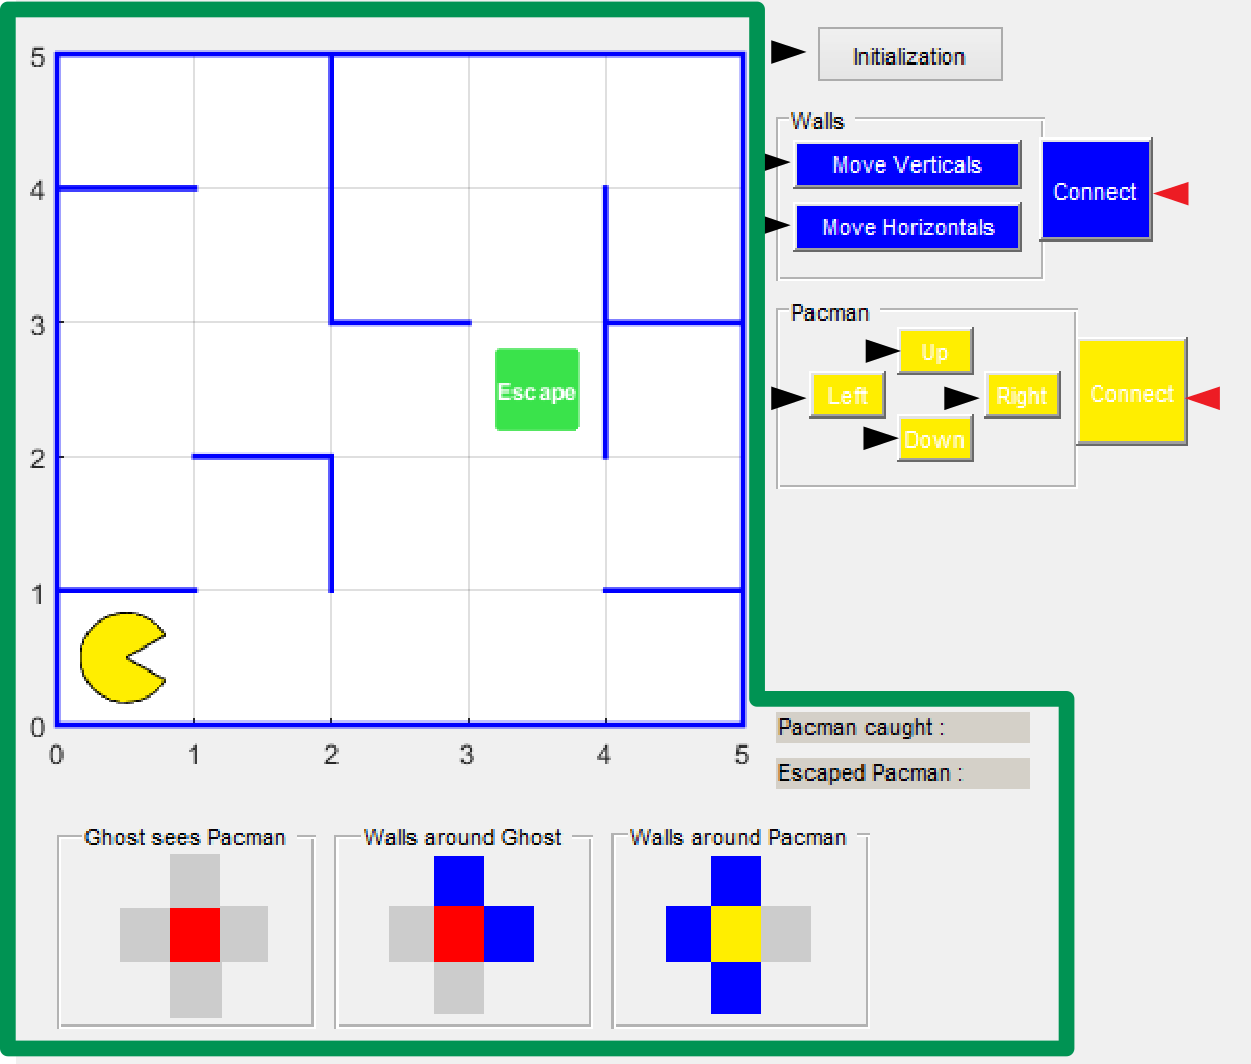
\includegraphics[width=8cm]{img_fig_lab.png}
\doxyfigcaption{button\textquotesingle{}s type of G\+UI}
\end{DoxyImage}
 This callback lanch update\+Connexion method of \hyperlink{class_wrapper}{Wrapper} class, which modify what command are automatic. 
\begin{DoxyParams}{Parameters}
{\em h\+Object} & handle to actived button \\
\hline
{\em eventdata} & reserved -\/ to be defined in a future version of M\+A\+T\+L\+AB \\
\hline
{\em handles} & structure with handles and user data (see G\+U\+I\+D\+A\+TA) \\
\hline
\end{DoxyParams}
\mbox{\Hypertarget{figure___laby_8m_a6d0378aadbd1b9c4ee65b7ce6c6f391c}\label{figure___laby_8m_a6d0378aadbd1b9c4ee65b7ce6c6f391c}} 
\index{figure\+\_\+\+Laby.\+m@{figure\+\_\+\+Laby.\+m}!create\+U\+I\+Escape@{create\+U\+I\+Escape}}
\index{create\+U\+I\+Escape@{create\+U\+I\+Escape}!figure\+\_\+\+Laby.\+m@{figure\+\_\+\+Laby.\+m}}
\subsubsection{\texorpdfstring{create\+U\+I\+Escape()}{createUIEscape()}}
{\footnotesize\ttfamily function create\+U\+I\+Escape (\begin{DoxyParamCaption}\item[{in}]{handles }\end{DoxyParamCaption})}



Creation of the graphical objects \char`\"{}escape\char`\"{}. 

The escape is created whit a rectangle and and text box. It\textquotesingle{}s stored into handles in \textquotesingle{}escape\textquotesingle{}. ~\newline

\begin{DoxyParams}{Parameters}
{\em handles} & structure with handles and user data (see G\+U\+I\+D\+A\+TA) \\
\hline
\end{DoxyParams}
\begin{DoxyReturn}{Returns}
h the updated structure with handles and user data (see G\+U\+I\+D\+A\+TA) 
\end{DoxyReturn}
\mbox{\Hypertarget{figure___laby_8m_a644de3f6b0431b1f28d5e9d15a8b002f}\label{figure___laby_8m_a644de3f6b0431b1f28d5e9d15a8b002f}} 
\index{figure\+\_\+\+Laby.\+m@{figure\+\_\+\+Laby.\+m}!create\+U\+I\+Pacman@{create\+U\+I\+Pacman}}
\index{create\+U\+I\+Pacman@{create\+U\+I\+Pacman}!figure\+\_\+\+Laby.\+m@{figure\+\_\+\+Laby.\+m}}
\subsubsection{\texorpdfstring{create\+U\+I\+Pacman()}{createUIPacman()}}
{\footnotesize\ttfamily function create\+U\+I\+Pacman (\begin{DoxyParamCaption}\item[{in}]{handles }\end{DoxyParamCaption})}



Creation of the graphical object \char`\"{}pacman\char`\"{}. 

The pacman is created by using the patch function and store into the handle in \textquotesingle{}pacman\textquotesingle{}. 
\begin{DoxyParams}{Parameters}
{\em handles} & structure with handles and user data (see G\+U\+I\+D\+A\+TA) \\
\hline
\end{DoxyParams}
\begin{DoxyReturn}{Returns}
h the updated structure with handles and user data (see G\+U\+I\+D\+A\+TA) 
\end{DoxyReturn}
\mbox{\Hypertarget{figure___laby_8m_ac7bdeec6012e991256f464a7e32155c2}\label{figure___laby_8m_ac7bdeec6012e991256f464a7e32155c2}} 
\index{figure\+\_\+\+Laby.\+m@{figure\+\_\+\+Laby.\+m}!create\+U\+I\+Walls@{create\+U\+I\+Walls}}
\index{create\+U\+I\+Walls@{create\+U\+I\+Walls}!figure\+\_\+\+Laby.\+m@{figure\+\_\+\+Laby.\+m}}
\subsubsection{\texorpdfstring{create\+U\+I\+Walls()}{createUIWalls()}}
{\footnotesize\ttfamily function create\+U\+I\+Walls (\begin{DoxyParamCaption}\item[{in}]{handles }\end{DoxyParamCaption})}



Creation of the graphical objects \char`\"{}walls\char`\"{}. 

The walls are created as two line elmenents matrix. They are stored into handles in \textquotesingle{}walls\textquotesingle{}. ~\newline
The first matrix is for the verticals walls and named \textquotesingle{}horizontals\textquotesingle{} and the second called \textquotesingle{}verticals\textquotesingle{} for the verticals walls.~\newline
All possible walls are created and it is by making them visible or invisible that they appear or disappear. 
\begin{DoxyParams}{Parameters}
{\em handles} & structure with handles and user data (see G\+U\+I\+D\+A\+TA) \\
\hline
\end{DoxyParams}
\begin{DoxyReturn}{Returns}
h the updated structure with handles and user data (see G\+U\+I\+D\+A\+TA) 
\end{DoxyReturn}
\mbox{\Hypertarget{figure___laby_8m_a9ab6a762fe20a58e9b1d54f8409c95d4}\label{figure___laby_8m_a9ab6a762fe20a58e9b1d54f8409c95d4}} 
\index{figure\+\_\+\+Laby.\+m@{figure\+\_\+\+Laby.\+m}!figure\+\_\+\+Laby@{figure\+\_\+\+Laby}}
\index{figure\+\_\+\+Laby@{figure\+\_\+\+Laby}!figure\+\_\+\+Laby.\+m@{figure\+\_\+\+Laby.\+m}}
\subsubsection{\texorpdfstring{figure\+\_\+\+Laby()}{figure\_Laby()}}
{\footnotesize\ttfamily function figure\+\_\+\+Laby (\begin{DoxyParamCaption}\item[{in}]{varargin }\end{DoxyParamCaption})}



\hyperlink{figure___laby_8m}{figure\+\_\+\+Laby.\+m} 

Script linked to the graphical interface whitch contain all the graphical functions. This file contain also the instance of \hyperlink{class_wrapper}{Wrapper} class. All the handles of graphical elements and instance of class are stored into the \char`\"{}handles\char`\"{} structure. function call when figure\+\_\+\+Laby si open. It\textquotesingle{}s initialize the UI. 
\begin{DoxyParams}{Parameters}
{\em varargin} & Several inputs. \\
\hline
\end{DoxyParams}
\begin{DoxyReturn}{Returns}
varargout Several Outputs. 
\end{DoxyReturn}
\mbox{\Hypertarget{figure___laby_8m_a60edd312a389dcd5feed96225a3f2d00}\label{figure___laby_8m_a60edd312a389dcd5feed96225a3f2d00}} 
\index{figure\+\_\+\+Laby.\+m@{figure\+\_\+\+Laby.\+m}!figure\+\_\+\+Laby\+\_\+\+Opening\+Fcn@{figure\+\_\+\+Laby\+\_\+\+Opening\+Fcn}}
\index{figure\+\_\+\+Laby\+\_\+\+Opening\+Fcn@{figure\+\_\+\+Laby\+\_\+\+Opening\+Fcn}!figure\+\_\+\+Laby.\+m@{figure\+\_\+\+Laby.\+m}}
\subsubsection{\texorpdfstring{figure\+\_\+\+Laby\+\_\+\+Opening\+Fcn()}{figure\_Laby\_OpeningFcn()}}
{\footnotesize\ttfamily function figure\+\_\+\+Laby\+\_\+\+Opening\+Fcn (\begin{DoxyParamCaption}\item[{in}]{h\+Object,  }\item[{in}]{eventdata,  }\item[{in}]{handles,  }\item[{in}]{varargin }\end{DoxyParamCaption})}



initialization function. 

It\textquotesingle{}s where is initialize the parameters of the labyrinth and all the commands in the section \char`\"{}\+I\+N\+I\+T\+I\+A\+L P\+A\+R\+A\+M\+E\+T\+E\+R\+S O\+F T\+H\+E L\+A\+B\+Y\+R\+I\+N\+T\+H  A\+N\+D T\+H\+E C\+O\+M\+M\+A\+N\+D\+S\char`\"{}. 
\begin{DoxyParams}{Parameters}
{\em h\+Object} & handle to figure \\
\hline
{\em eventdata} & reserved -\/ to be defined in a future version of M\+A\+T\+L\+AB \\
\hline
{\em handles} & structure with handles and user data (see G\+U\+I\+D\+A\+TA) \\
\hline
{\em varargin} & command line arguments to figure\+\_\+\+Laby (see V\+A\+R\+A\+R\+G\+IN) \\
\hline
\end{DoxyParams}
\mbox{\Hypertarget{figure___laby_8m_a819520b7fe35fe3b612cbe16336f65c3}\label{figure___laby_8m_a819520b7fe35fe3b612cbe16336f65c3}} 
\index{figure\+\_\+\+Laby.\+m@{figure\+\_\+\+Laby.\+m}!figure\+\_\+\+Laby\+\_\+\+Output\+Fcn@{figure\+\_\+\+Laby\+\_\+\+Output\+Fcn}}
\index{figure\+\_\+\+Laby\+\_\+\+Output\+Fcn@{figure\+\_\+\+Laby\+\_\+\+Output\+Fcn}!figure\+\_\+\+Laby.\+m@{figure\+\_\+\+Laby.\+m}}
\subsubsection{\texorpdfstring{figure\+\_\+\+Laby\+\_\+\+Output\+Fcn()}{figure\_Laby\_OutputFcn()}}
{\footnotesize\ttfamily function figure\+\_\+\+Laby\+\_\+\+Output\+Fcn (\begin{DoxyParamCaption}\item[{in}]{h\+Object,  }\item[{in}]{eventdata,  }\item[{in}]{handles }\end{DoxyParamCaption})}



Automatic generated function by G\+UI. 


\begin{DoxyParams}{Parameters}
{\em h\+Object} & handle to figure \\
\hline
{\em eventdata} & reserved -\/ to be defined in a future version of M\+A\+T\+L\+AB \\
\hline
{\em handles} & structure with handles and user data (see G\+U\+I\+D\+A\+TA) \\
\hline
\end{DoxyParams}
\begin{DoxyReturn}{Returns}
varargout cell array for returning output args (see V\+A\+R\+A\+R\+G\+O\+UT); 
\end{DoxyReturn}
\mbox{\Hypertarget{figure___laby_8m_a1a18fd2ef966c79b4687a62f38657cc6}\label{figure___laby_8m_a1a18fd2ef966c79b4687a62f38657cc6}} 
\index{figure\+\_\+\+Laby.\+m@{figure\+\_\+\+Laby.\+m}!is\+One@{is\+One}}
\index{is\+One@{is\+One}!figure\+\_\+\+Laby.\+m@{figure\+\_\+\+Laby.\+m}}
\subsubsection{\texorpdfstring{is\+One()}{isOne()}}
{\footnotesize\ttfamily function is\+One (\begin{DoxyParamCaption}\item[{in}]{bool\+Cond }\end{DoxyParamCaption})}



Return the string \textquotesingle{}on\textquotesingle{} if the input is 1 else, return the string \textquotesingle{}off\textquotesingle{}. 


\begin{DoxyParams}{Parameters}
{\em bool\+Cond} & integer to convert \\
\hline
\end{DoxyParams}
\begin{DoxyReturn}{Returns}
str\+On\+Off Returned string. Can be worth \char`\"{}on\char`\"{} or \char`\"{}off\char`\"{}. 
\end{DoxyReturn}
\mbox{\Hypertarget{figure___laby_8m_a1a026f7304bcc541b6cf3fcb38ef0716}\label{figure___laby_8m_a1a026f7304bcc541b6cf3fcb38ef0716}} 
\index{figure\+\_\+\+Laby.\+m@{figure\+\_\+\+Laby.\+m}!reset\+U\+I\+Connection@{reset\+U\+I\+Connection}}
\index{reset\+U\+I\+Connection@{reset\+U\+I\+Connection}!figure\+\_\+\+Laby.\+m@{figure\+\_\+\+Laby.\+m}}
\subsubsection{\texorpdfstring{reset\+U\+I\+Connection()}{resetUIConnection()}}
{\footnotesize\ttfamily function reset\+U\+I\+Connection (\begin{DoxyParamCaption}\item[{in}]{handles }\end{DoxyParamCaption})}



Reset all commands connections to unconnected. 

This function reset wrapper\textquotesingle{}s property and graphical element to unconnected state. 
\begin{DoxyParams}{Parameters}
{\em handles} & structure with handles and user data (see G\+U\+I\+D\+A\+TA) \\
\hline
\end{DoxyParams}
\begin{DoxyReturn}{Returns}
h the updated structure with handles and user data (see G\+U\+I\+D\+A\+TA) 
\end{DoxyReturn}
\mbox{\Hypertarget{figure___laby_8m_a13e8832f06299624ef0f167e80097f4c}\label{figure___laby_8m_a13e8832f06299624ef0f167e80097f4c}} 
\index{figure\+\_\+\+Laby.\+m@{figure\+\_\+\+Laby.\+m}!ui\+\_\+\+Callback@{ui\+\_\+\+Callback}}
\index{ui\+\_\+\+Callback@{ui\+\_\+\+Callback}!figure\+\_\+\+Laby.\+m@{figure\+\_\+\+Laby.\+m}}
\subsubsection{\texorpdfstring{ui\+\_\+\+Callback()}{ui\_Callback()}}
{\footnotesize\ttfamily function ui\+\_\+\+Callback (\begin{DoxyParamCaption}\item[{in}]{h\+Object,  }\item[{in}]{eventdata,  }\item[{in}]{handles }\end{DoxyParamCaption})}



Callback for all the action\textquotesingle{}s buttons (see detailed explications). 

in the following image, buttons marked with a black arrow lanch this Callback. ~\newline

\begin{DoxyImage}
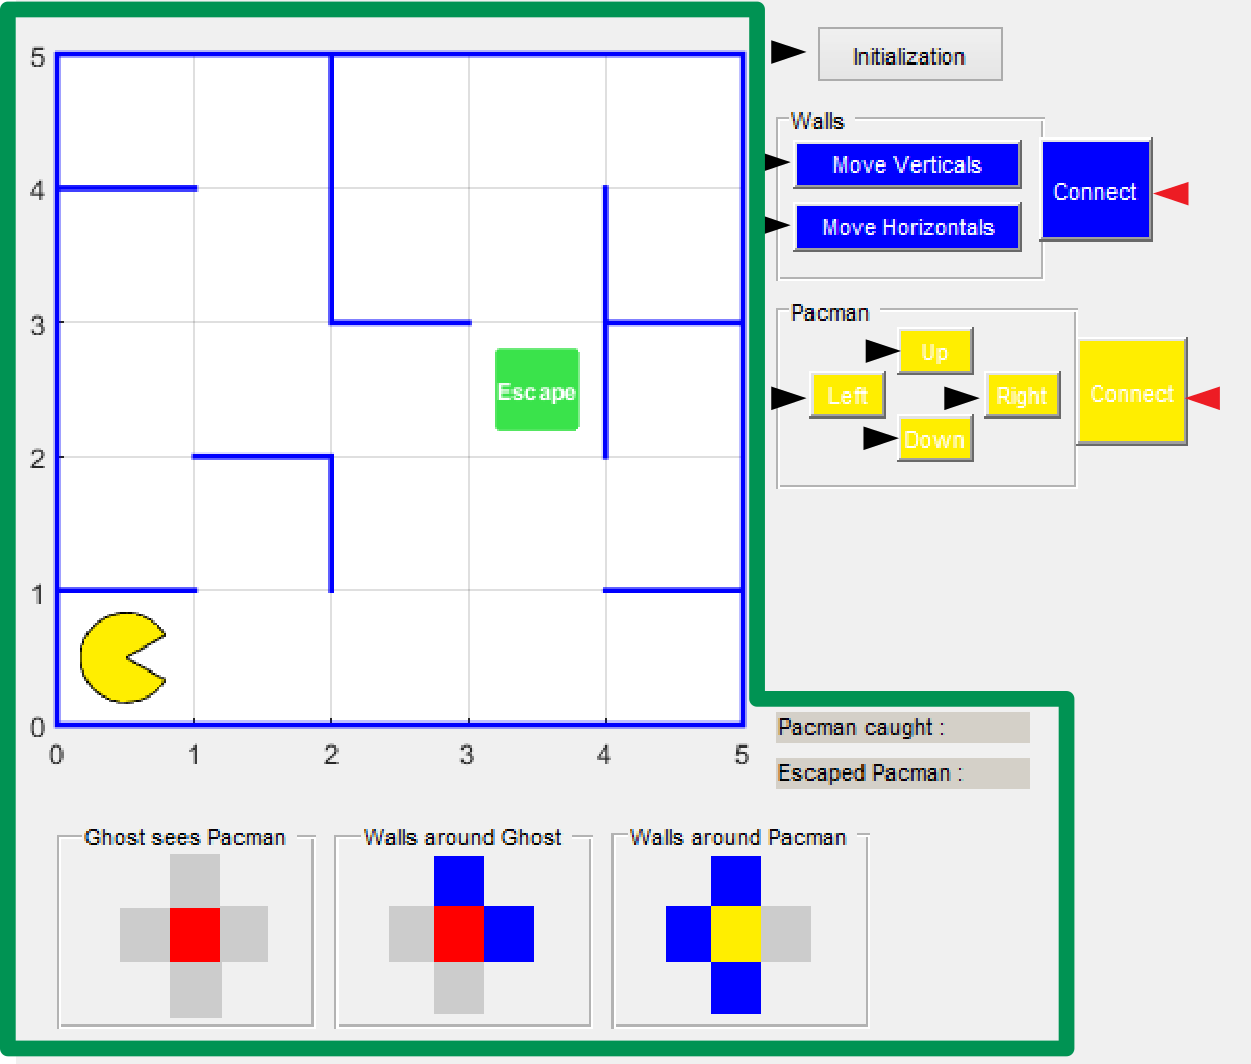
\includegraphics[width=10cm]{img_fig_lab.png}
\doxyfigcaption{button\textquotesingle{}s type of G\+UI}
\end{DoxyImage}
 This callback lanch orderer method of \hyperlink{class_wrapper}{Wrapper} class, which allows the simulation to evolve. 
\begin{DoxyParams}{Parameters}
{\em h\+Object} & handle to actived button \\
\hline
{\em eventdata} & reserved -\/ to be defined in a future version of M\+A\+T\+L\+AB \\
\hline
{\em handles} & structure with handles and user data (see G\+U\+I\+D\+A\+TA) \\
\hline
\end{DoxyParams}
\mbox{\Hypertarget{figure___laby_8m_ac8b43d61d9c22654239e5aee49117c0e}\label{figure___laby_8m_ac8b43d61d9c22654239e5aee49117c0e}} 
\index{figure\+\_\+\+Laby.\+m@{figure\+\_\+\+Laby.\+m}!update\+Presence\+Detector\+Display@{update\+Presence\+Detector\+Display}}
\index{update\+Presence\+Detector\+Display@{update\+Presence\+Detector\+Display}!figure\+\_\+\+Laby.\+m@{figure\+\_\+\+Laby.\+m}}
\subsubsection{\texorpdfstring{update\+Presence\+Detector\+Display()}{updatePresenceDetectorDisplay()}}
{\footnotesize\ttfamily function update\+Presence\+Detector\+Display (\begin{DoxyParamCaption}\item[{in}]{element\+To\+Set,  }\item[{in}]{bool\+Condition }\end{DoxyParamCaption})}



Change the background color of the graphical Element according to the state of the binary condition. 

This function, with a boolean condition (integer) and a handle to a graphical element update the background color. ~\newline
If the Boolean value is 1, the background color turns blue, otherwise it will be gray. 
\begin{DoxyParams}{Parameters}
{\em element\+To\+Set} & handle to the graphical element. \\
\hline
{\em bool\+Condition} & input boolean condition store in a integer. \\
\hline
\end{DoxyParams}
\mbox{\Hypertarget{figure___laby_8m_a9ec6541b09e277ad9513cd8352d7f4ad}\label{figure___laby_8m_a9ec6541b09e277ad9513cd8352d7f4ad}} 
\index{figure\+\_\+\+Laby.\+m@{figure\+\_\+\+Laby.\+m}!update\+UI@{update\+UI}}
\index{update\+UI@{update\+UI}!figure\+\_\+\+Laby.\+m@{figure\+\_\+\+Laby.\+m}}
\subsubsection{\texorpdfstring{update\+U\+I()}{updateUI()}}
{\footnotesize\ttfamily function update\+UI (\begin{DoxyParamCaption}\item[{in}]{handles,  }\item[{in}]{out }\end{DoxyParamCaption})}



This function update all graphicals element who can change. 

With the input called \textquotesingle{}out\textquotesingle{}, this function lanch all the functions who update a specific graphical element. 
\begin{DoxyParams}{Parameters}
{\em handles} & Structure with handles and user data (see G\+U\+I\+D\+A\+TA) \\
\hline
{\em out} & Cell who contain all informations needed from the wrapper for update the graphical interface. \\
\hline
\end{DoxyParams}
\mbox{\Hypertarget{figure___laby_8m_a87c1d45c5bfdbbda7c7e018944352f4e}\label{figure___laby_8m_a87c1d45c5bfdbbda7c7e018944352f4e}} 
\index{figure\+\_\+\+Laby.\+m@{figure\+\_\+\+Laby.\+m}!update\+U\+I\+Active\+Cammand@{update\+U\+I\+Active\+Cammand}}
\index{update\+U\+I\+Active\+Cammand@{update\+U\+I\+Active\+Cammand}!figure\+\_\+\+Laby.\+m@{figure\+\_\+\+Laby.\+m}}
\subsubsection{\texorpdfstring{update\+U\+I\+Active\+Cammand()}{updateUIActiveCammand()}}
{\footnotesize\ttfamily function update\+U\+I\+Active\+Cammand (\begin{DoxyParamCaption}\item[{in}]{handles }\end{DoxyParamCaption})}



Update visibility of control panel, connection and step button. 

This function show or hide the control\textquotesingle{}s panels and the connection\textquotesingle{}s buttons according whit who will move. It also show step button if a command is connected. ~\newline
Example \+: if is pacman time to move and command is not connected, this function hide walls and step element and show pacman one\textquotesingle{}s. 
\begin{DoxyParams}{Parameters}
{\em handles} & structure with handles and user data (see G\+U\+I\+D\+A\+TA) \\
\hline
\end{DoxyParams}
\mbox{\Hypertarget{figure___laby_8m_a38cb193f7c7132094881ec92e1e1f1ae}\label{figure___laby_8m_a38cb193f7c7132094881ec92e1e1f1ae}} 
\index{figure\+\_\+\+Laby.\+m@{figure\+\_\+\+Laby.\+m}!update\+U\+I\+Button@{update\+U\+I\+Button}}
\index{update\+U\+I\+Button@{update\+U\+I\+Button}!figure\+\_\+\+Laby.\+m@{figure\+\_\+\+Laby.\+m}}
\subsubsection{\texorpdfstring{update\+U\+I\+Button()}{updateUIButton()}}
{\footnotesize\ttfamily function update\+U\+I\+Button (\begin{DoxyParamCaption}\item[{in}]{handles }\end{DoxyParamCaption})}



Show the needed moving buttons. 

This function show the direction\textquotesingle{}s buttons allows by the output informations of model\+Laby and hide the others one. 
\begin{DoxyParams}{Parameters}
{\em handles} & structure with handles and user data (see G\+U\+I\+D\+A\+TA) \\
\hline
\end{DoxyParams}
\mbox{\Hypertarget{figure___laby_8m_a0bc4f0536957330137cf68c471dd7275}\label{figure___laby_8m_a0bc4f0536957330137cf68c471dd7275}} 
\index{figure\+\_\+\+Laby.\+m@{figure\+\_\+\+Laby.\+m}!update\+U\+I\+Escape@{update\+U\+I\+Escape}}
\index{update\+U\+I\+Escape@{update\+U\+I\+Escape}!figure\+\_\+\+Laby.\+m@{figure\+\_\+\+Laby.\+m}}
\subsubsection{\texorpdfstring{update\+U\+I\+Escape()}{updateUIEscape()}}
{\footnotesize\ttfamily function update\+U\+I\+Escape (\begin{DoxyParamCaption}\item[{in}]{element\+To\+Set,  }\item[{in}]{bool\+State }\end{DoxyParamCaption})}



Update graphical static text block about escape status. 

This function, with the output of the wrapper, show \textquotesingle{}Yes\textquotesingle{} in the static text block where is write \char`\"{}\+Espcaped Pacman \+: \char`\"{} if the pacman is on the escape case. ~\newline
In the green box in the following image. 
\begin{DoxyImage}
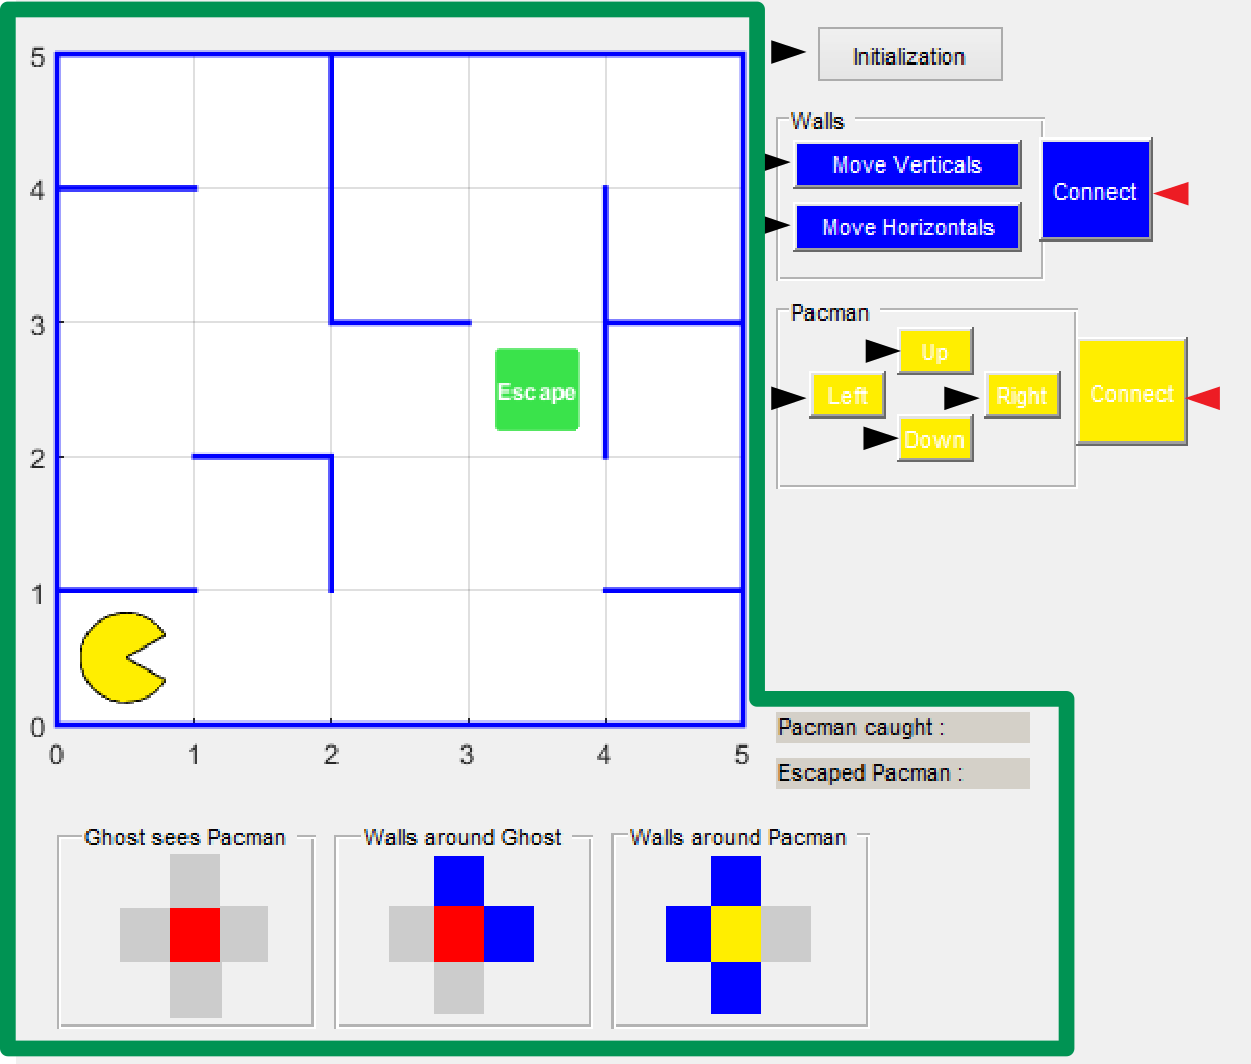
\includegraphics[width=8cm]{img_fig_lab.png}
\doxyfigcaption{graphicals elements}
\end{DoxyImage}
 
\begin{DoxyParams}{Parameters}
{\em element\+To\+Set} & handle to the graphical object for escape status. \\
\hline
{\em bool\+State} & Value of the escape output of wrapper. (1 if pacman is escaped, else 0.) \\
\hline
\end{DoxyParams}
\mbox{\Hypertarget{figure___laby_8m_abe5f5974e5080c6ec025b754bd247b24}\label{figure___laby_8m_abe5f5974e5080c6ec025b754bd247b24}} 
\index{figure\+\_\+\+Laby.\+m@{figure\+\_\+\+Laby.\+m}!update\+U\+I\+Player@{update\+U\+I\+Player}}
\index{update\+U\+I\+Player@{update\+U\+I\+Player}!figure\+\_\+\+Laby.\+m@{figure\+\_\+\+Laby.\+m}}
\subsubsection{\texorpdfstring{update\+U\+I\+Player()}{updateUIPlayer()}}
{\footnotesize\ttfamily function update\+U\+I\+Player (\begin{DoxyParamCaption}\item[{in}]{handles,  }\item[{in}]{str\+Player,  }\item[{in}]{position }\end{DoxyParamCaption})}



Update graphical place of a player (only pacman in this case). 

This function, with the actual position (present in the handles) and the new one as a input, move object. ~\newline
The dynamics of movement is defined by this foncion $ out(t) = \frac{\frac{om+1}{om*e^{cv*t}+1}-1}{om} $ for $ t \in [0,1]$, $ om = 72.89105$ and $ cv = -11.27357 $. 
\begin{DoxyImage}
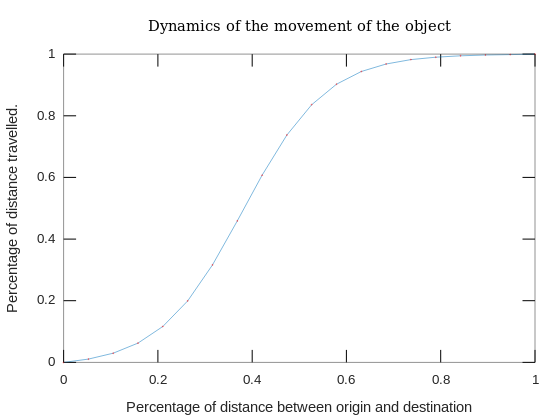
\includegraphics[width=8cm]{obj_dynamic.png}
\doxyfigcaption{Dynamics of movement}
\end{DoxyImage}
 
\begin{DoxyParams}{Parameters}
{\em str\+Player} & String contain the exact name of the object to move. \\
\hline
{\em position} & new position of the object. format \+: \mbox{[}x y\mbox{]} \\
\hline
{\em handles} & structure with handles and user data (see G\+U\+I\+D\+A\+TA) \\
\hline
\end{DoxyParams}
\mbox{\Hypertarget{figure___laby_8m_aeeec55039fa4664a85aa8407d992f621}\label{figure___laby_8m_aeeec55039fa4664a85aa8407d992f621}} 
\index{figure\+\_\+\+Laby.\+m@{figure\+\_\+\+Laby.\+m}!update\+U\+I\+Walls@{update\+U\+I\+Walls}}
\index{update\+U\+I\+Walls@{update\+U\+I\+Walls}!figure\+\_\+\+Laby.\+m@{figure\+\_\+\+Laby.\+m}}
\subsubsection{\texorpdfstring{update\+U\+I\+Walls()}{updateUIWalls()}}
{\footnotesize\ttfamily function update\+U\+I\+Walls (\begin{DoxyParamCaption}\item[{in}]{walls\+UI,  }\item[{in}]{vert\+Walls,  }\item[{in}]{horiz\+Walls }\end{DoxyParamCaption})}



Update graphicals elements for the walls. 

This function, with the output of the wrapper, update displayed part and hided part of the walls. 
\begin{DoxyParams}{Parameters}
{\em walls\+UI} & handle to the matrixs of graphicals elements for walls. \\
\hline
{\em vert\+Walls} & Corresponding part of output of wrapper for verticals walls.. \\
\hline
{\em horiz\+Walls} & Corresponding part of output of wrapper for horizontals walls. \\
\hline
\end{DoxyParams}
\mbox{\Hypertarget{figure___laby_8m_a1d96d5c1168a9db6b7530ed1e117697d}\label{figure___laby_8m_a1d96d5c1168a9db6b7530ed1e117697d}} 
\index{figure\+\_\+\+Laby.\+m@{figure\+\_\+\+Laby.\+m}!update\+U\+I\+Walls\+Around@{update\+U\+I\+Walls\+Around}}
\index{update\+U\+I\+Walls\+Around@{update\+U\+I\+Walls\+Around}!figure\+\_\+\+Laby.\+m@{figure\+\_\+\+Laby.\+m}}
\subsubsection{\texorpdfstring{update\+U\+I\+Walls\+Around()}{updateUIWallsAround()}}
{\footnotesize\ttfamily function update\+U\+I\+Walls\+Around (\begin{DoxyParamCaption}\item[{in}]{handles,  }\item[{in}]{str\+Element,  }\item[{in}]{walls\+Around }\end{DoxyParamCaption})}



Update graphical elements for walls around pacman. 

This function, with the output of the wrapper, update color of gray squares that represents walls presence around the pacman. 
\begin{DoxyParams}{Parameters}
{\em str\+Element} & common part of the name of the handle to the graphical object for walls around pacman. \\
\hline
{\em walls\+Around} & Value of the corresponding part of output of wrapper. \\
\hline
{\em handles} & structure with handles and user data (see G\+U\+I\+D\+A\+TA) \\
\hline
\end{DoxyParams}

\hypertarget{main_8m}{}\section{main.\+m File Reference}
\label{main_8m}\index{main.\+m@{main.\+m}}

\hypertarget{_model_laby_8m}{}\section{Model\+Laby.\+m File Reference}
\label{_model_laby_8m}\index{Model\+Laby.\+m@{Model\+Laby.\+m}}
\subsection*{Classes}
\begin{DoxyCompactItemize}
\item 
class \hyperlink{class_model_laby}{Model\+Laby}
\begin{DoxyCompactList}\small\item\em Class which contains the \char`\"{}fmg\char`\"{} structure of the labyrinth for 1 player. \end{DoxyCompactList}\end{DoxyCompactItemize}

\hypertarget{_model_pacman_8m}{}\section{Model\+Pacman.\+m File Reference}
\label{_model_pacman_8m}\index{Model\+Pacman.\+m@{Model\+Pacman.\+m}}


Contain Pacman movement control.  


\subsection*{Classes}
\begin{DoxyCompactItemize}
\item 
class \hyperlink{class_model_pacman}{Model\+Pacman}
\begin{DoxyCompactList}\small\item\em Input \+: Possible Pacman\textquotesingle{}s moves \mbox{[}Up Down Left Right\mbox{]} ~\newline
 0 = move not possible ; 1 = move possible ~\newline
 ( Wout\{7\} )~\newline
~\newline
 Output \+: Pacman\textquotesingle{}s moves 1 \+: pacman\+Left\+But, ( Wout(3) )~\newline
 2 \+: pacman\+Up\+But, ( Wout(1) )~\newline
 3 \+: pacman\+Right\+But, ( Wout(4) )~\newline
 4 \+: pacman\+Down\+But , ( Wout(2) )~\newline
 ( Win( 4\+:7) of wrapper ) ~\newline
. \end{DoxyCompactList}\end{DoxyCompactItemize}


\subsection{Detailed Description}
Contain Pacman movement control. 


\hypertarget{_model_s_e_d_8m}{}\section{Model\+S\+E\+D.\+m File Reference}
\label{_model_s_e_d_8m}\index{Model\+S\+E\+D.\+m@{Model\+S\+E\+D.\+m}}
\subsection*{Classes}
\begin{DoxyCompactItemize}
\item 
class \hyperlink{class_model_s_e_d}{Model\+S\+ED}
\end{DoxyCompactItemize}

\hypertarget{_model_walls_8m}{}\section{Model\+Walls.\+m File Reference}
\label{_model_walls_8m}\index{Model\+Walls.\+m@{Model\+Walls.\+m}}
\subsection*{Classes}
\begin{DoxyCompactItemize}
\item 
class \hyperlink{class_model_walls}{Model\+Walls}
\end{DoxyCompactItemize}

\hypertarget{set_color_8m}{}\section{set\+Color.\+m File Reference}
\label{set_color_8m}\index{set\+Color.\+m@{set\+Color.\+m}}
\subsection*{Functions}
\begin{DoxyCompactItemize}
\item 
\hyperlink{_plan__desuma_functions_8m_ac2ffb26d6f42d3bbcd7847b0873403f4}{function} \hyperlink{set_color_8m_a2e19e78cd7b120fed65bf33d319f5bee}{set\+Color} (in img, in img\+Ref, in colors, in indice)
\end{DoxyCompactItemize}


\subsection{Function Documentation}
\mbox{\Hypertarget{set_color_8m_a2e19e78cd7b120fed65bf33d319f5bee}\label{set_color_8m_a2e19e78cd7b120fed65bf33d319f5bee}} 
\index{set\+Color.\+m@{set\+Color.\+m}!set\+Color@{set\+Color}}
\index{set\+Color@{set\+Color}!set\+Color.\+m@{set\+Color.\+m}}
\subsubsection{\texorpdfstring{set\+Color()}{setColor()}}
{\footnotesize\ttfamily \hyperlink{_plan__desuma_functions_8m_ac2ffb26d6f42d3bbcd7847b0873403f4}{function} set\+Color (\begin{DoxyParamCaption}\item[{in}]{img,  }\item[{in}]{img\+Ref,  }\item[{in}]{colors,  }\item[{in}]{indice }\end{DoxyParamCaption})}


\hypertarget{_simulation_8m}{}\section{Simulation.\+m File Reference}
\label{_simulation_8m}\index{Simulation.\+m@{Simulation.\+m}}


Script to launch the labyrinth simulation.  




\subsection{Detailed Description}
Script to launch the labyrinth simulation. 


\hypertarget{_stop_condition_8m}{}\section{Stop\+Condition.\+m File Reference}
\label{_stop_condition_8m}\index{Stop\+Condition.\+m@{Stop\+Condition.\+m}}
\subsection*{Classes}
\begin{DoxyCompactItemize}
\item 
class \hyperlink{class_stop_condition}{Stop\+Condition}
\begin{DoxyCompactList}\small\item\em Class used to manage shutdown conditions. \end{DoxyCompactList}\end{DoxyCompactItemize}

\hypertarget{test_u_i_8m}{}\section{test\+U\+I.\+m File Reference}
\label{test_u_i_8m}\index{test\+U\+I.\+m@{test\+U\+I.\+m}}

\hypertarget{_t_h_eplan_8m}{}\section{T\+H\+Eplan.\+m File Reference}
\label{_t_h_eplan_8m}\index{T\+H\+Eplan.\+m@{T\+H\+Eplan.\+m}}

\hypertarget{visupacman_8m}{}\section{visupacman.\+m File Reference}
\label{visupacman_8m}\index{visupacman.\+m@{visupacman.\+m}}

\hypertarget{visupacman2_8m}{}\section{visupacman2.\+m File Reference}
\label{visupacman2_8m}\index{visupacman2.\+m@{visupacman2.\+m}}

\hypertarget{walls_border_8m}{}\section{walls\+Border.\+m File Reference}
\label{walls_border_8m}\index{walls\+Border.\+m@{walls\+Border.\+m}}
\subsection*{Functions}
\begin{DoxyCompactItemize}
\item 
\hyperlink{_plan__desuma_functions_8m_ac2ffb26d6f42d3bbcd7847b0873403f4}{function} \hyperlink{walls_border_8m_a80033169a4bb46973c96b0f9bda4a37f}{walls\+Border} (in walls)
\end{DoxyCompactItemize}


\subsection{Function Documentation}
\mbox{\Hypertarget{walls_border_8m_a80033169a4bb46973c96b0f9bda4a37f}\label{walls_border_8m_a80033169a4bb46973c96b0f9bda4a37f}} 
\index{walls\+Border.\+m@{walls\+Border.\+m}!walls\+Border@{walls\+Border}}
\index{walls\+Border@{walls\+Border}!walls\+Border.\+m@{walls\+Border.\+m}}
\subsubsection{\texorpdfstring{walls\+Border()}{wallsBorder()}}
{\footnotesize\ttfamily \hyperlink{_plan__desuma_functions_8m_ac2ffb26d6f42d3bbcd7847b0873403f4}{function} walls\+Border (\begin{DoxyParamCaption}\item[{in}]{walls }\end{DoxyParamCaption})}


\hypertarget{_wrapper_8m}{}\section{Wrapper.\+m File Reference}
\label{_wrapper_8m}\index{Wrapper.\+m@{Wrapper.\+m}}
\subsection*{Classes}
\begin{DoxyCompactItemize}
\item 
class \hyperlink{class_wrapper}{Wrapper}
\begin{DoxyCompactList}\small\item\em Connects all models to the display function. \end{DoxyCompactList}\end{DoxyCompactItemize}

%--- End generated contents ---

% Index
\backmatter
\newpage
\phantomsection
\clearemptydoublepage
\addcontentsline{toc}{chapter}{Index}
\printindex

\end{document}
